% arara: lualatex: { synctex: on, shell: off }
% arara: biber
% arara: lualatex: { synctex: on, shell: off }
% arara: sumatrapdf
\documentclass[../main.tex]{subfiles}

\begin{document}

\begin{table}[!ht]
    \caption{HHV of Ethanol, Butanol Isomers, and Gasoline}
    \label{tab:buoh-heats}
    \begin{tabular}{*{4}{c}}
        \toprule
        Compound & Ethanol \cite{Afeefy2014} & Butanol Isomers \cite{Afeefy2014} & Gasoline \cite{Davis2013} \\
        \midrule
        HHV [\si[per-mode = symbol]{\mega\joule\per\kilo\gram}] & 29.67 & $\approx 36$ & 48.46 \\
        \bottomrule
    \end{tabular}
\end{table}

\begin{figure}[!ht]
    \ffigbox{%
        \begin{subfloatrow}[4]
            \ffigbox
                {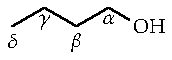
\includegraphics[width=3cm]{03-Butanol/nbuoh-skeletal}}%
                {\caption{\nBuOH{}}\label{fig:nbuoh-skeletal}}%
            \ffigbox
                {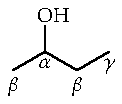
\includegraphics[width=3cm]{03-Butanol/sbuoh-skeletal}}%
                {\caption{\sBuOH{}}\label{fig:sbuoh-skeletal}}%
            \ffigbox
                {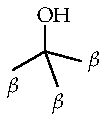
\includegraphics[height=2.5cm]{03-Butanol/tbuoh-skeletal}}%
                {\caption{\tBuOH{}}\label{fig:tbuoh-skeletal}}%
            \ffigbox
                {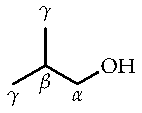
\includegraphics[width=3cm]{03-Butanol/ibuoh-skeletal}}%
                {\caption{\iBuOH{}}\label{fig:ibuoh-skeletal}}%
        \end{subfloatrow}
    }%
    {\caption{Skeletal structures of the butanol isomers}
    \label{fig:buoh-isomers}}
\end{figure}

\section{Structure of the Butanol Isomers}
\label{sec:butanol-isomers}

Butanol is the four carbon alcohol, and has four isomers:
\nBuOH{} (1-butanol);
\sBuOH{} (2-butanol);
\tBuOH{} (2-methyl-2-propanol); and
\iBuOH{} (2-methyl-1-propanol).
The skeletal structures of the four isomers are shown in
\cref{fig:buoh-isomers}. The carbon atoms in the skeleton are
labeled according to their distance from the hydroxyl moeity; the
$\alpha$ carbon is the closest to the hydroxyl, followed by $\beta$,
$\gamma$, and $\delta$ carbons. Not all of the butanols have all of
the types of carbons listed here, due to varying chain lengths. For
instance, \tBuOH{} has one $\alpha$ carbon (not labeled), three $\beta$
carbons, and no $\gamma$ or $\delta$ carbons.


Three of the butanol isomers can be produced
by biological pathways (\textit{n}-, \textit{s}-, and \iBuOH{})
\cite{Nigam2011,Smith2010}, making them candidates for the ``second-generation''
of biofuels \cite{Harvey2011,Nigam2011}. Although \tBuOH{} does not have
an identified biological production pathway, it has commercial significance
as an octane enhancer. In addition, the four isomers of butanol represent
the smallest alcohol system with all four types of branching in the skeleton.
This makes them excellent candidates to build kinetic models that can be
extended to larger alcohols with similar structures.

\Cref{tab:buoh-heats} shows a comparison of the higher heating value of
the butanol isomers with ethanol and gasoline. The higher energy density
of the butanol isomers allows them to be blended in gasoline in higher
proportions and reduces the volumetric fuel economy (e.g.\ mpg) impact
of replacing gasoline with biofuels.

\section{Experimental Procedure}
\label{sec:buoh-proc}

The reactants used in this study, along with their purities, are shown in
\cref{tab:buoh-expts}. To determine the relative proportions of each
reactant in the mixture, the absolute mass of fuel, the equivalence ratio
($\phi$), and the oxidizer ratio ($X_{O_2}:X_{\mathrm{inert}}$, where $X$
indicates mole fraction) are specified. \textit{s}- and \textit{i}-Butanol are
liquid at room temperature and have relatively low vapor pressure; therefore,
each is massed in a syringe to within \SI{0.01}{g} of the specified
value. \textit{t}-Butanol is solid at room temperature (melting point: \SI{25}{\celsius}),
and is melted before being handled in the same procedure as the other fuels.
The \SI{17}{\liter} mixing tank is vacuumed to an ultimate pressure less than \SI{5}{Torr} prior
to the injection of the liquid fuel through a septum. Proportions of O$_2$ and
N$_2$ are added manometrically at room temperature. The preheat temperature of
the RCM is set above the saturation point for each fuel to ensure complete
vaporization. A magnetic stirrer mixes the reactants. The temperature inside
the mixing tank is allowed to equilibrate for approximately \SI{1.5}{\hour}.

This approach to mixture preparation has been validated in several previous
studies by withdrawing gas samples from the mixing tank and analyzing the
contents by GC/MS \cite{Weber2011}, GC-FID \cite{Kumar2009}, and GC-TCD
\cite{Das2012}. These studies have verified the concentration of
\nBuOH{}, \textit{n}-decane, and water, respectively. In addition,
both the work by \textcite{Kumar2009} on \textit{n}-decane and the study of
\textcite{Weber2011} on \nBuOH{} confirmed that there was no fuel
decomposition over the course of a typical set of experiments. Furthermore,
within this study, each new mixture preparation is checked against previously
tested conditions to ensure reproducibility.

\Cref{tab:buoh-expts} shows the experimental conditions considered in this
study. The compressed pressure conditions have been chosen to match the
previous \nBuOH{} study \cite{Weber2011}, but also to provide data in
regions not covered extensively in previous work. In addition, the fuel loading
conditions have been chosen to complement previous work; the studies by
\textcite{Stranic2012} and \textcite{Moss2008} used relatively dilute mixtures,
so we have included higher fuel loading conditions. Furthermore, the compressed
temperature conditions we have studied ($T_C=\SIrange{715}{910}{\kelvin}$) have not been examined
in any other study, to our knowledge.

\begin{table}
    \caption{Experimental Conditions and Reactant Purities}
    \label{tab:buoh-expts}
    \begin{tabular}{*{7}{c}}
    \toprule
    \multicolumn{5}{c}{Reactant (Purity)} & \multirow{3}[0]{*}{\linebreakcell{Equivalence \\ Ratio \\ $\phi$}} & \multirow{3}[0]{*}{\linebreakcell{Compressed \\ Pressure \\ $P_C$ (bar)}} \\
    \cmidrule{1-5}
    \linebreakcell{\sBuOH{} \\ (\SI{99.99}{\percent})} & \linebreakcell{\iBuOH{} \\ (\SI{99.99}{\percent})} & \linebreakcell{\tBuOH{} \\ (\SI{99.99}{\percent})} & \linebreakcell{O$_2$ \\ (\SI{99.999}{\percent})} & \linebreakcell{N$_2$ \\ (\SI{99.995}{\percent})} & & \\
    \cmidrule{1-5}
    \multicolumn{5}{c}{Mole Percentage}   & & \\
    \midrule
    3.38 &      &      & 20.30 & 76.32 & 1.0 & 15 \\
    3.38 &      &      & 20.30 & 76.32 & 1.0 & 30 \\
         & 3.38 &      & 20.30 & 76.32 & 1.0 & 15 \\
         & 3.38 &      & 20.30 & 76.32 & 1.0 & 30 \\
         &      & 3.38 & 20.30 & 76.32 & 1.0 & 15 \\
         &      & 3.38 & 20.30 & 76.32 & 1.0 & 30 \\
         &      & 1.72 & 20.65 & 77.63 & 0.5 & 30 \\
         &      & 6.54 & 19.63 & 73.83 & 2.0 & 30 \\
         & 1.72 &      & 20.65 & 77.63 & 0.5 & 15 \\
         & 1.72 &      & 20.65 & 77.63 & 0.5 & 30 \\
         & 3.38 &      & 40.60 & 56.02 & 0.5 & 15 \\
         & 3.38 &      & 40.60 & 56.02 & 0.5 & 30 \\
         & 3.38 &      & 10.15 & 86.47 & 2.0 & 30 \\
         & 3.38 &      & 10.15 & 86.47 & 2.0 & 30 \\
    \bottomrule
    \end{tabular}
\end{table}

\section{Experimental Results}
\subsection{Comparison of Butanol Isomers Ignition}
\label{sec:buoh-expts}

\Cref{fig:buoh-15bar} shows the ignition delays of the four isomers of
butanol measured in the RCM, at compressed pressure of $P_C=\SI{15}{\bar}$ for
stoichiometric mixture in air. The dashed line for each isomer is a least
squares fit to the data. The vertical error bars are two standard deviations
of the measurements of the ignition delay. The standard deviation is computed
based on all the runs at a particular compressed temperature and pressure
condition, as discussed in \cref{sec:ign-delay-def}. The uncertainty in
$T_C$ was estimated in \cref{sec:unc-alcohol} to be approximately
\SIrange{2}{3}{\percent}.

\Cref{fig:buoh-15bar} demonstrates the differences in reactivity between
the isomers for stoichiometric fuel/air mixtures at compressed pressure
$P_C=\SI{15}{\bar}$. \textit{n}-Butanol is clearly the most reactive, followed by
\textit{s}- and \iBuOH{}, which have very similar reactivities in
this temperature and pressure range. \textit{t}-Butanol is the least reactive.

The order of reactivity found in the RCM at \SI{15}{\bar} agrees with the ST
study at higher temperatures (approximately \SIrange{1275}{1667}{\kelvin}) and lower pressure
(\SI{1.5}{atm}) by \textcite{Stranic2012} but differs slightly from the studies of
\textcite{Moss2008} who measured ignition delays in a ST near \SI{1.5}{atm}
and between \SIrange{1275}{1400}{\kelvin}, and \textcite{Veloo2011a} who measured
atmospheric-pressure laminar flame speeds. In particular, \textcite{Moss2008}
and \textcite{Veloo2011a} found distinct differences in reactivity between
\textit{s}- and \iBuOH{}, but the present study and the study by
\textcite{Stranic2012} found that they were nearly indistinguishable in terms
of reactivity under the conditions investigated. In addition,
\textcite{Stranic2012} noted some disagreement between their ST
ignition data and the data of \textcite{Moss2008} but their attempts to isolate
the cause could not discern what the difference might be caused by.

Further, the order of the reactivity of the butanol isomers shows complex
temperature and pressure dependence. This is demonstrated by the results shown
in \cref{fig:buoh-30bar}. In \cref{fig:buoh-30bar}, the order of
reactivity is different than in \cref{fig:buoh-15bar}, where the only
variation between the plots is the compressed pressure; in
\cref{fig:buoh-30bar} the compressed pressure is $P_C=\SI{30}{\bar}$.
\cref{fig:buoh-30bar} shows \iBuOH{} to be the least reactive,
\sBuOH{} to be less reactive than but similar to \tBuOH{},
and \nBuOH{} to be the most reactive. Interestingly, the results of
the ST study by \textcite{Stranic2012} differ from those in the current
study at higher pressure, despite the agreement at lower pressure. In their
study, \textcite{Stranic2012} found \textit{i}- and \nBuOH{} to have
similar reactivity near \SI{43}{atm} in the temperature range of \SIrange{1020}{1280}{\kelvin},
whereas in the present study we find \iBuOH{} to be the least
reactive of all four isomers at a pressure of \SI{30}{\bar} and over the temperature
range (\SIrange{715}{910}{\kelvin}) investigated.

\begin{figure}
    \begin{floatrow}
    \ffigbox
        {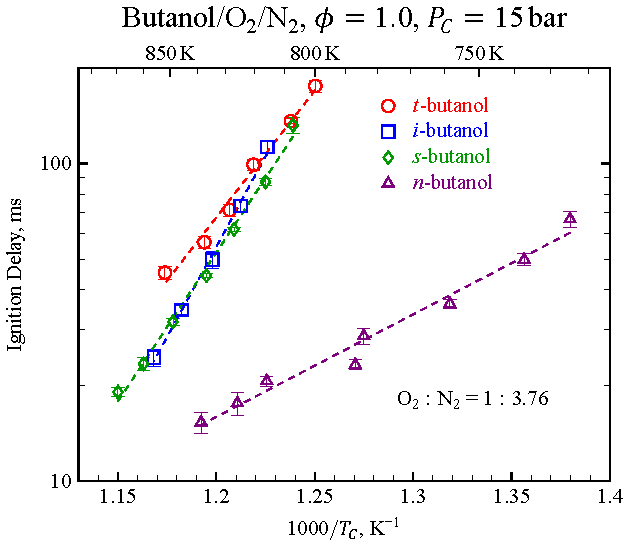
\includegraphics[width=7.9cm]{03-Butanol/buoh-15bar}}
        {\caption{Ignition delays of the four isomers of butanol at compressed
            pressure $P_C=\SI{15}{\bar}$. Dashed lines are least squares fits to the
            data.}
        \label{fig:buoh-15bar}}
    \ffigbox
        {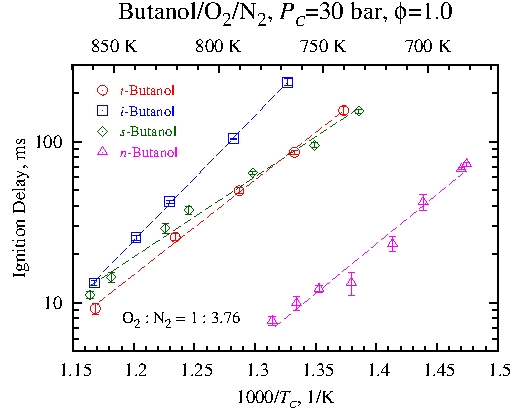
\includegraphics[width=7.9cm]{03-Butanol/buoh-30bar}}
        {\caption{Ignition delays of the four isomers of butanol at compressed
            pressure $P_C=\SI{30}{\bar}$. Dashed lines are least squares fits to the
            data.}
        \label{fig:buoh-30bar}}
    \end{floatrow}
\end{figure}

\subsection{Ignition of \textit{t}-Butanol}
\label{sec:tbuoh-ignition}

The fact that \tBuOH{} becomes relatively more reactive than
\textit{i}- and \sBuOH{} as pressure increases is surprising at first
glance, and the reasons are not immediately apparent. Closer examination of the
pressure traces for each experiment gives one clue as to the cause of the
increased reactivity. \Cref{fig:tbuoh-15bar} shows the pressure traces for
the \tBuOH{} experiments at \SI{15}{\bar} for stoichiometric mixtures in
air. It is evident that there is some pre-ignition heat release, because the
reactive pressure trace diverges from the non-reactive case prior to the
ignition event. Of the other isomers of butanol, only \nBuOH{} shows
any visible heat release prior to the main ignition event at \SI{15}{\bar}.

\Cref{fig:tbuoh-phi10} shows the pressure traces for \tBuOH{}
experiments at \SI{30}{\bar} for stoichiometric mixtures in air. The effect of
pre-ignition heat release is even more striking in this figure, with
substantial changes in the slope of the pressure trace during the reactive
runs. Comparison to the pressure traces of the other isomers once again shows
that the magnitude of the pre-ignition heat release for \tBuOH{} is
much greater. Despite the appearance of early pressure rise, which is typically
indicative of two-stage ignition and low temperature chain branching, we do not
find a negative temperature coefficient region in terms of the ignition delay
response for any \tBuOH{} experiments. Therefore, we adopt the phrase
``pre-ignition heat release'' rather than ``two-stage ignition'' in this work.

\begin{figure}
    \begin{floatrow}
    \ffigbox
        {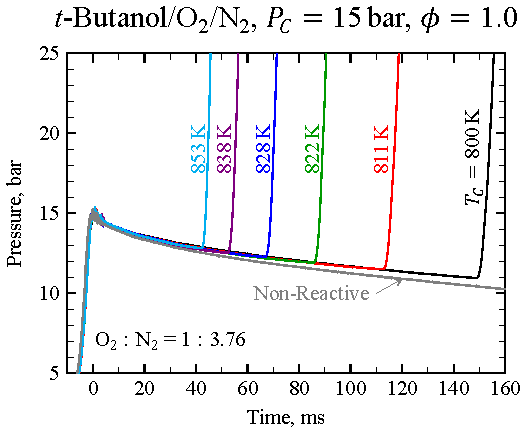
\includegraphics[width=7.9cm]{03-Butanol/tbuoh-15bar}}
        {\caption{Pressure traces of the \SI{15}{\bar} \tBuOH{} experiments,
            in stoichiometric air.}
        \label{fig:tbuoh-15bar}}
    \ffigbox
        {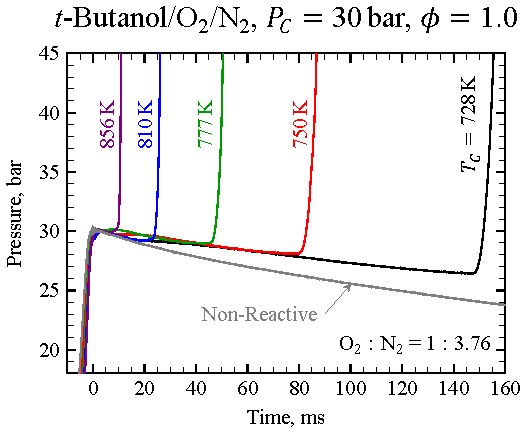
\includegraphics[width=7.9cm]{03-Butanol/tbuoh-phi10}}
        {\caption{Pressure traces of the \SI{30}{\bar} \tBuOH{} experiments,
            in stoichiometric air.}
        \label{fig:tbuoh-phi10}}
    \end{floatrow}
\end{figure}

In an effort to understand the reactions causing the pre-ignition heat release,
further experiments are conducted for \tBuOH{} at $P_C=\SI{30}{\bar}$, for
equivalence ratios of 0.5 and 2.0 in air. \Cref{fig:tbuoh-delays} shows
Arrhenius plots of the ignition delays for the three equivalence ratios. As
with the previous \nBuOH{} experiments at \SI{15}{\bar} \cite{Weber2011}
$\phi=\num{0.5}$ is the least reactive and $\phi=\num{2.0}$ is the most reactive. The
slopes are similar, indicating that the overall activation energies are similar
for the conditions investigated.

\begin{figure}
    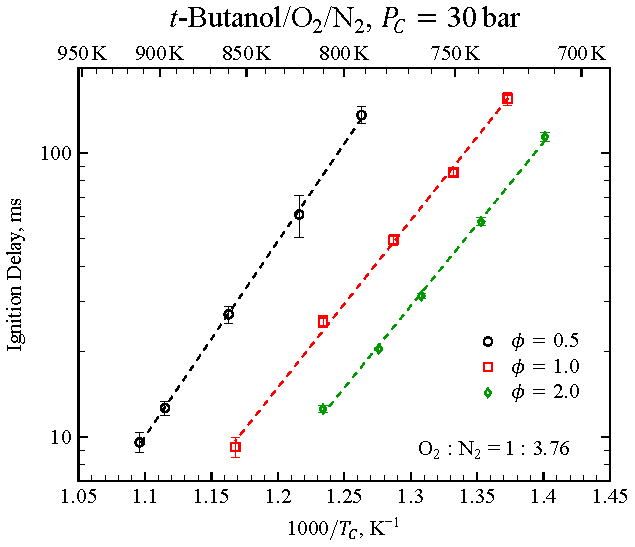
\includegraphics[width=12cm]{03-Butanol/tbuoh-delays}
    \caption{Ignition delays of three equivalence ratios of \tBuOH{}
    in air, for $P_C=\SI{30}{\bar}$. Lines represent least squares fits to the data.}
    \label{fig:tbuoh-delays}
\end{figure}

A more interesting comparison is of the pressure traces of the three
equivalence ratios. It is clear from \cref{fig:tbuoh-phi10,fig:tbuoh-phi05,%
fig:tbuoh-phi20} that there are qualitative differences in the pre-ignition
heat release between the three equivalence ratios. This is most likely
due to the effect of the increased (reduced) fuel mole fraction in the
$\phi=\num{2.0}$ ($\phi=\num{0.5}$) case, since the mole fraction of
fuel is changed by +\SI{93}{\percent} (-\SI{49}{\percent}) compared to the $\phi=\num{1.0}$ case, while the
mole fraction of oxygen changes by only -\SI{3}{\percent} (+\SI{2}{\percent}) compared to the $\phi=\num{1.0}$
case, as shown in \cref{tab:buoh-expts}. Therefore, it appears that the
qualitative change in pre-ignition behavior is due to the change of fuel mole
fraction, where higher fuel loading promotes pre-ignition heat release.

\begin{figure}
    \begin{floatrow}
    \ffigbox
        {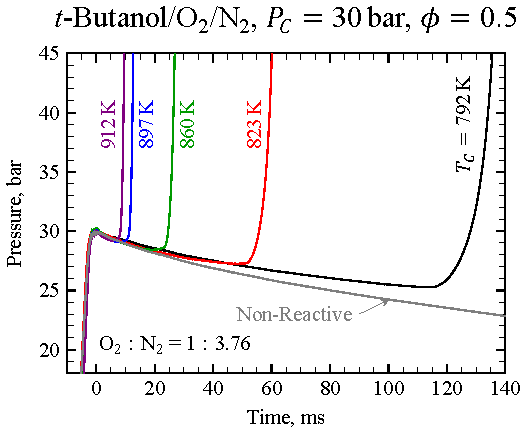
\includegraphics[width=7.9cm]{03-Butanol/tbuoh-phi05}}
        {\caption{Pressure traces of the \SI{30}{\bar} \tBuOH{} experiments,
            $\phi=\num{0.5}$ in air.}
        \label{fig:tbuoh-phi05}}
    \ffigbox
        {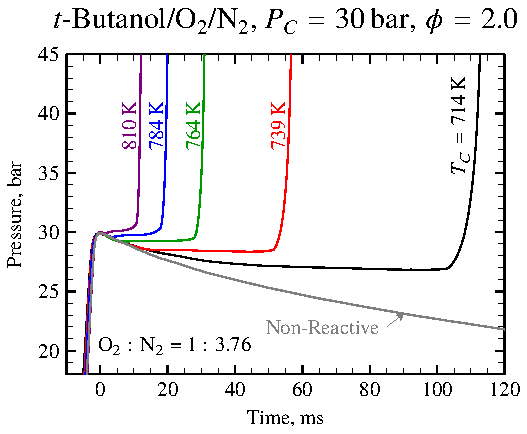
\includegraphics[width=7.9cm]{03-Butanol/tbuoh-phi20}}
        {\caption{Pressure traces of the \SI{30}{\bar} \tBuOH{} experiments,
            $\phi=\num{2.0}$ in air.}
        \label{fig:tbuoh-phi20}}
    \end{floatrow}
\end{figure}

\subsection{Ignition of \textit{i}-Butanol}
\label{sec:ibuoh-ignition}

The experimental ignition delays of \iBuOH{} measured at
$P_C=\SIlist{15;30}{\bar}$ and $\phi=0.5$ in oxygen/nitrogen air are shown in
\cref{fig:ibuoh-expts}. The error bars are equal to twice the standard
deviation of all the runs at that condition. The lines are curve fits to
the data. The circles represent the \SI{15}{\bar} data, while the
squares represent the \SI{30}{\bar} data. Also shown in
\cref{fig:ibuoh-expts} are the experimental ignition delays presented in
\cref{sec:buoh-expts} at $\phi=1.0$ and $P_C=\SIlist{15;30}{\bar}$. The
$\phi=0.5$ cases are shown in blue and the $\phi=1.0$ cases are shown in
red.

For both equivalence ratios, the \SI{15}{\bar} cases are less reactive
than the \SI{30}{\bar} cases, as judged by the inverse of the
ignition delay. Furthermore, in comparing the $\phi=1.0$ data to the
$\phi=0.5$ data at the same compressed pressure, it is seen that the
strong equivalence ratio dependence of the ignition delays previously
measured for two other isomers of butanol, \nBuOH{} \cite{Weber2011} and
\tBuOH{} (\cref{sec:tbuoh-ignition}), is also present for \iBuOH{}.

\begin{figure}
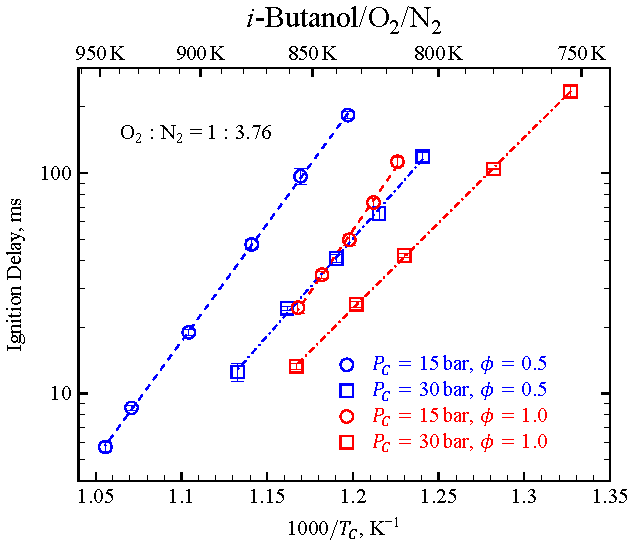
\includegraphics[width=11cm]{03-Butanol/ibuoh-expts}
\caption{Comparison of the experimentally measured ignition delays of
         \iBuOH{} at two compressed pressures, $P_C=\SI{15}{\bar}$
         (circles) and $P_C=\SI{30}{\bar}$ (squares), and two equivalence
         ratios, $\phi=0.5$ (blue) and $\phi=1.0$ (red).}
\label{fig:ibuoh-expts}
\end{figure}

\Cref{fig:ibuoh-15o2expt,fig:ibuoh-30o2expt} show the ignition delays of
\iBuOH{} at three equivalence ratios $\phi=\numlist{0.5;1.0;2.0}$ and
$P_C=\SIlist{15;30}{\bar}$ respectively. In these figures, the equivalence
ratio is varied by holding the initial fuel mole fraction constant and
varying the oxygen and nitrogen mole fractions. The ignition delay
of \iBuOH{} depends strongly on the initial oxygen mole fraction, similar
to the trend shown for \nBuOH{} \cite{Weber2011}.

\begin{figure}
    \begin{floatrow}
    \ffigbox
        {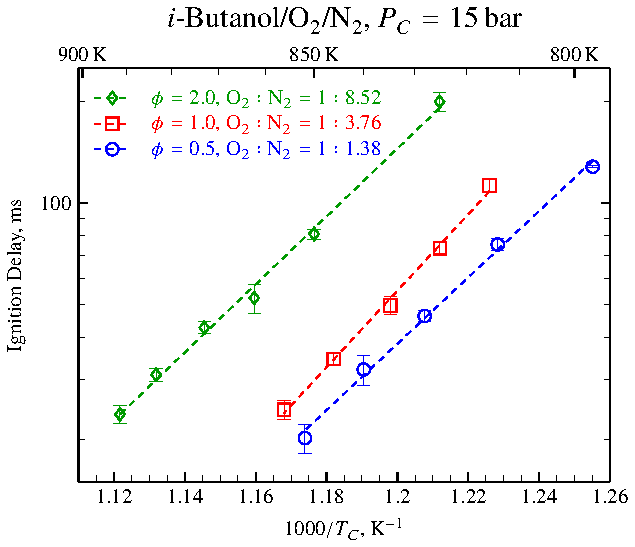
\includegraphics[width=7.9cm]{03-Butanol/ibuoh-15o2expt}}
        {\caption{Comparison of the experimentally measured ignition
        delays of \iBuOH{} at three equivalence ratios and $P_C=\SI{15}{\bar}$.
        The equivalence ratio is changed by varying the initial oxygen
        mole fraction at constant initial fuel mole fraction.}
        \label{fig:ibuoh-15o2expt}}
    \ffigbox
        {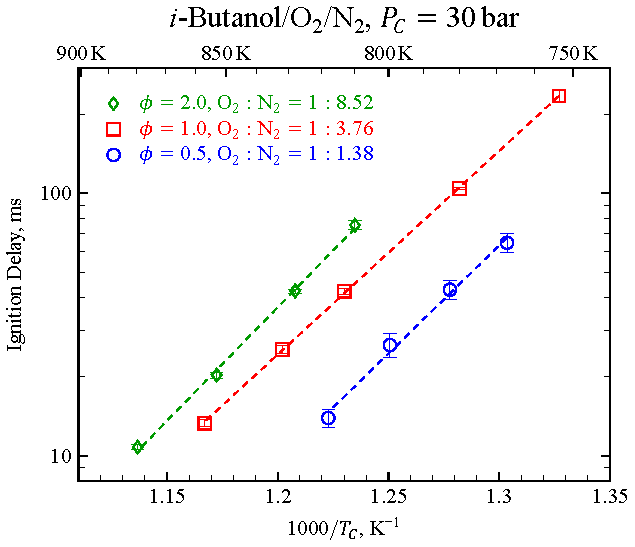
\includegraphics[width=7.9cm]{03-Butanol/ibuoh-30o2expt}}
        {\caption{Comparison of the experimentally measured ignition
        delays of \iBuOH{} at three equivalence ratios and $P_C=\SI{30}{\bar}$.
        The equivalence ratio is changed by varying the initial oxygen
        mole fraction at constant initial fuel mole fraction.}
        \label{fig:ibuoh-30o2expt}}
    \end{floatrow}
\end{figure}

\section{Simulation Results}
\subsection{Comparison of Simulated Butanol Isomers Ignition}
\label{sec:buoh-sims}

Simulations are performed with the kinetic mechanism from
\textcite{Sarathy2012} denoted as the Sarathy et al.\ mechanism.
Other recent mechanisms, such as the mechanism from
\textcite{Frassoldati2012} do not include low temperature chemistry and are
therefore unable to reproduce the low-temperature ignition delays measured in
this study. The study by \textcite{Sarathy2012} validated their model for a
wide set of the existing experimental data. In terms of ignition delays, this
included the data from the study of \textcite{Stranic2012} up to \SI{48}{atm}, our
previous study on \nBuOH{} \cite{Weber2011}, and the data being
published in this study at \SI{15}{\bar}. Importantly, the mechanism of
\textcite{Sarathy2012} was validated only for the \SI{15}{\bar} RCM data for all four
isomers, but not the \SI{30}{\bar} data also being published here. The MIT mechanism
\cite{Hansen2013,Merchant2013} was validated for \iBuOH{}
experiments, including pyrolysis and low pressure premixed flames; although the
model includes all four isomers of butanol as reactants, it has not been
optimized for any of the isomers except \iBuOH{}.

\Cref{fig:buoh-15sim,fig:buoh-30sim} show comparison of the
VPRO simulations with the experimental data using the mechanism of
\textcite{Sarathy2012}. As \textcite{Sarathy2012} showed in their work (and as
we show here in \cref{fig:buoh-15sim}), they found good agreement of the
model predictions with the present RCM data at \SI{15}{\bar}. At $P_C=\SI{30}{\bar}$
(\cref{fig:buoh-30sim}), similar degree of agreement is found for
\tBuOH{} and \sBuOH{} compared to $P_C=\SI{15}{\bar}$, although
the \sBuOH{} results are under-predicted at high temperature and
over-predicted at low temperature. While the model of \textcite{Sarathy2012} is
able to well capture the overall activation energy of \iBuOH{}, it
under-predicts the experimental data by about a factor of \numrange{2}{3}. The
\nBuOH{} data are over-predicted by a factor of about 1.5.
Nevertheless, this agreement is quite good, especially considering that the
model is not validated for these conditions.

\begin{figure}
    \begin{floatrow}
    \ffigbox
        {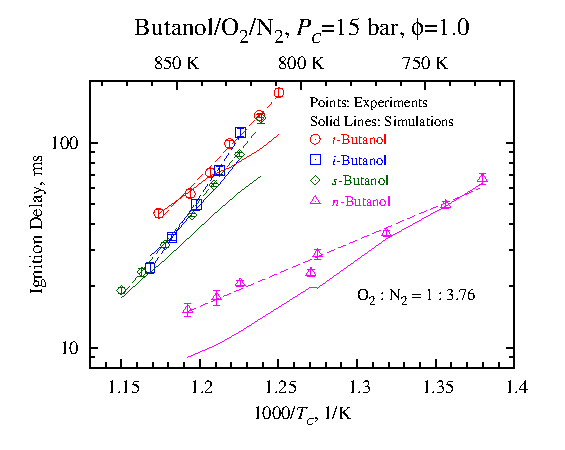
\includegraphics[width=7.9cm]{03-Butanol/buoh-15sim}}
        {\caption{$P_C=\SI{15}{\bar}$, stoichiometric mixtures in air. Comparison of
            VPRO simulations using the kinetic mechanism of
            \textcite{Sarathy2012} with experimental ignition delays.}
        \label{fig:buoh-15sim}}
    \ffigbox
        {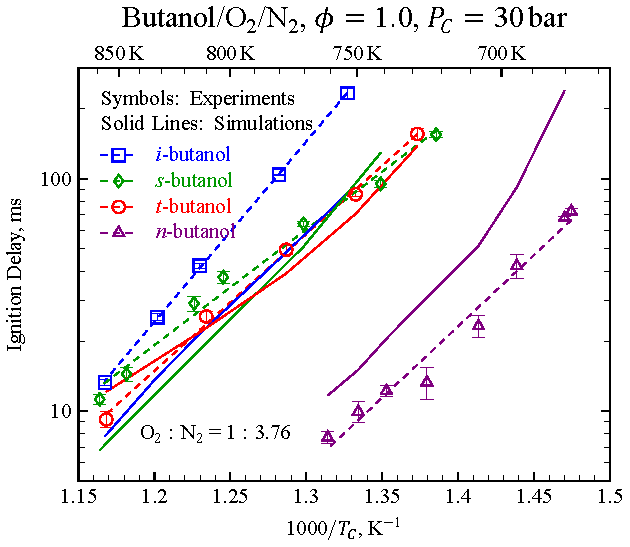
\includegraphics[width=7.9cm]{03-Butanol/buoh-30sim}}
        {\caption{$P_C=\SI{30}{\bar}$, stoichiometric mixtures in air. Comparison of
            VPRO simulations using the kinetic mechanism of
            \textcite{Sarathy2012} with experimental ignition delays.}
        \label{fig:buoh-30sim}}
    \end{floatrow}
\end{figure}

\subsection{Simulated \textit{t}-Butanol Ignition}

The agreement of the mechanism by \textcite{Sarathy2012} with the
off-stoichiometric mixtures of \tBuOH{} is also quite good, as shown
in \cref{fig:tbuoh-sims}. \Cref{fig:tbuoh-05press,fig:tbuoh-10press,,%The double comma is necessary to prevent compression
fig:tbuoh-20press} show more detailed comparisons
of the simulated pressure traces and the experimental results, for similar
temperatures at the three equivalence ratios, respectively. Clearly, the
simulations also exhibit some pre-ignition heat release. In general, the
simulations qualitatively predict the pre-ignition heat release behavior at all
three equivalence ratios. The $\phi=\num{0.5}$ case has the least heat release and
the $\phi=\num{2.0}$ case has the most. Although the simulations are unable to match
the heat release behavior quantitatively, they match the experimental ignition
delays quite well. Considering the model is not validated for this temperature,
pressure, and equivalence ratio regime, the mismatch of the pre-ignition
behavior may not be of critical importance, depending on the application.

\begin{figure}
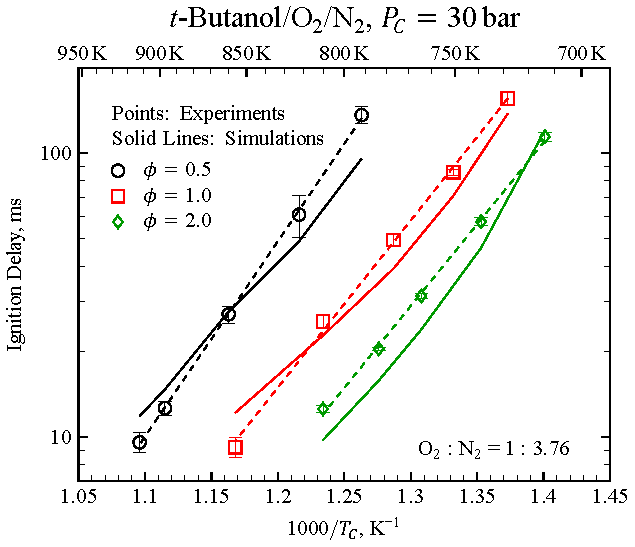
\includegraphics[width=11cm]{03-Butanol/tbuoh-sims}
\caption{Comparison of the simulations using the kinetic mechanism of
\textcite{Sarathy2012} for three equivalence ratio mixtures of
\tBuOH{} in air at $P_C=\SI{30}{\bar}$.}
\label{fig:tbuoh-sims}
\end{figure}

\begin{figure}
    \ffigbox{%
    \begin{subfloatrow}[3]
        \ffigbox[\FBwidth]
            {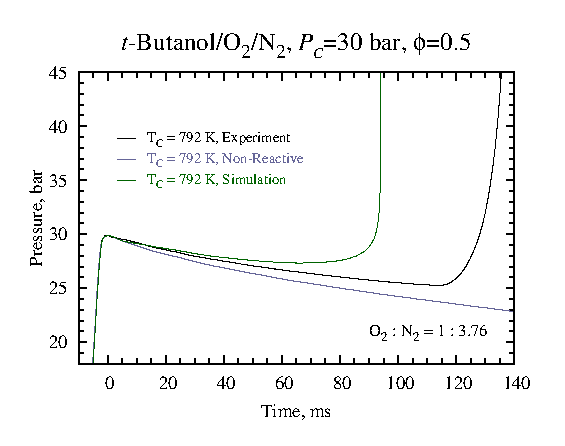
\includegraphics[width=5.2cm]{03-Butanol/tbuoh-05press}}
            {\caption{$\phi=\num{0.5}$ in air.}
            \label{fig:tbuoh-05press}}
        \ffigbox[\FBwidth]
            {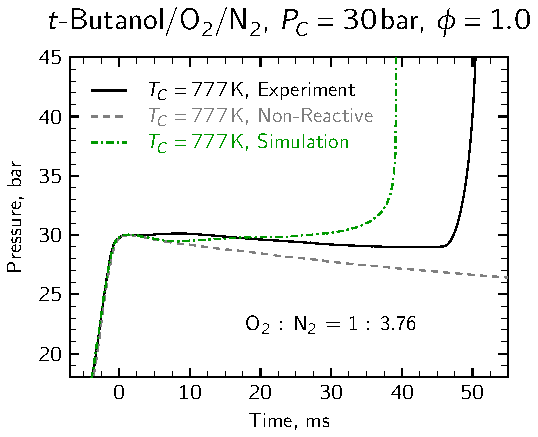
\includegraphics[width=5.2cm]{03-Butanol/tbuoh-10press}}
            {\caption{$\phi=\num{1.0}$ in air.}
            \label{fig:tbuoh-10press}}
        \ffigbox[\FBwidth]
            {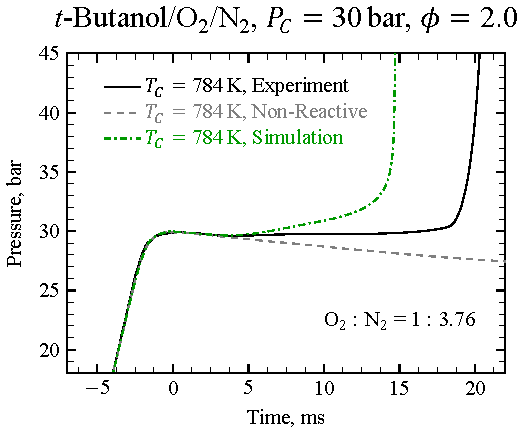
\includegraphics[width=5.2cm]{03-Butanol/tbuoh-20press}}
            {\caption{$\phi=\num{2.0}$ in air.}
            \label{fig:tbuoh-20press}}
    \end{subfloatrow}
    }%
    {\caption{Pressure traces of selected
     \tBuOH{} experiments compared with the corresponding
     non-reactive and simulated traces, using the mechanism of
     \textcite{Sarathy2012}.}
    }
\end{figure}

\subsection{Simulated \textit{i}-Butanol Ignition}
\label{sec:ibuoh-sims}

In addition to the model by \textcite{Sarathy2012} which is validated for
all four isomers of butanol, a kinetic model for the combustion of
\iBuOH{} has been developed and presented by \textcite{Hansen2013,
Merchant2013}. This model has been validated for species profiles
measured in a low-pressure, premixed flame by \textcite{Hansen2013},
an atmospheric pressure diffusion flame by \textcite{Grana2010}, and a
doped methane flame by \textcite{McEnally2005}, ignition delays measured
by \textcite{Stranic2012}, JSR species profiles measured by
\textcite{Togbe2010}, laminar flame speeds measured by
\textcite{Veloo2011a,Liu2011a}, and species profiles from a pyrolysis
reactor \textcite{Merchant2013}.

Recently, the \iBuOH{} model developed by \textcite{Hansen2013,
Merchant2013} has been updated with new reaction rates and pathways.
The updates are detailed in the work of \textcite{Weber2013a}. The
primary updates were to add detailed low-temperature peroxy pathways
involving \iBuOH{} and its primary radicals. This model is still undergoing
validation, but is presented here as the state-of-the-art in butanol
modeling. This kinetic model will be referred to as the MIT mechanism.

In \cref{fig:buoh-mit}, VPRO simulations at \SIlist{15;30}{\bar} using
the Sarathy et al.\ mechanism \cite{Sarathy2012} and the MIT mechanism
\cite{Weber2013a} are shown for \iBuOH{}. Some conditions using the MIT
mechanism did not ignite during the simulated time (approximately
\SI{800}{\milli\second}), so those points are not shown in
\cref{fig:buoh-mit}. The mechanism by Sarathy et al.\ is in better
agreement with the experiments at \SI{15}{\bar} than the MIT model. At
\SI{30}{\bar} the MIT model over-predicts the ignition delay---as at
\SI{15}{\bar}---while the Sarathy et al.\ mechanism under-predicts the
ignition delay.

\begin{figure}
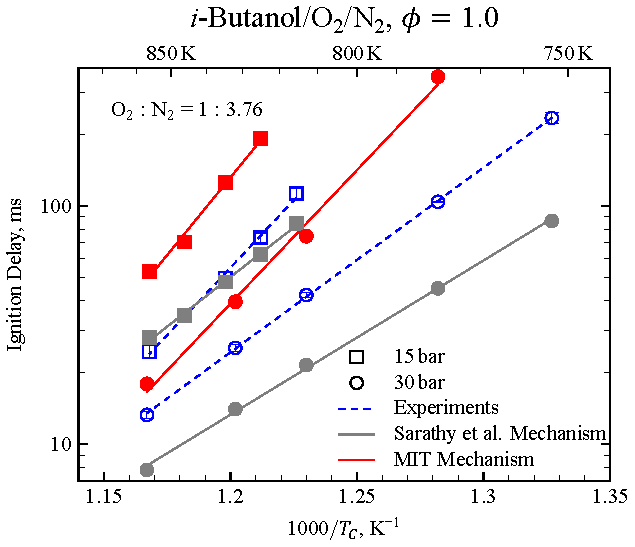
\includegraphics[width=11cm]{03-Butanol/buoh-mit}
\caption{Comparison of VPRO simulations using the kinetic mechanism of
\textcite{Sarathy2012} (gray) and the MIT mechanism
\cite{Hansen2013,Merchant2013} (red) with the experimental
ignition delay results (blue) for stoichiometric mixtures of
\iBuOH{} in air at $P_C=\SI{15}{\bar}$ (squares) and $P_C=\SI{30}{\bar}$
(circles).}
\label{fig:buoh-mit}
\end{figure}

\Cref{fig:ibuoh-15o2sim,fig:ibuoh-30o2sim} show comparisons of VPRO
simulations using the MIT mechanism with the experimental data at three
equivalence ratios with constant initial fuel mole fraction. In general,
the model is unable to predict the oxygen concentration dependence of the
ignition delays. A similar result was found for the comparison of
\nBuOH{} experiments with a model constructed using the same principles
as the present model for \iBuOH{} \cite{Weber2011}. Moreover, comparing
the experimental results with modeling results using the mechanism of
\textcite{Sarathy2012} reveals a similar qualitative discrepancy,
although the Sarathy et al.\ model tends to under-predict the experimental
ignition delays whereas the MIT model tends to over-predict the experimental
values. The reason for these diverging predictions will be explored and
discussed in \cref{sec:ibuoh-discussion}.

\begin{figure}
    \begin{floatrow}
    \ffigbox
        {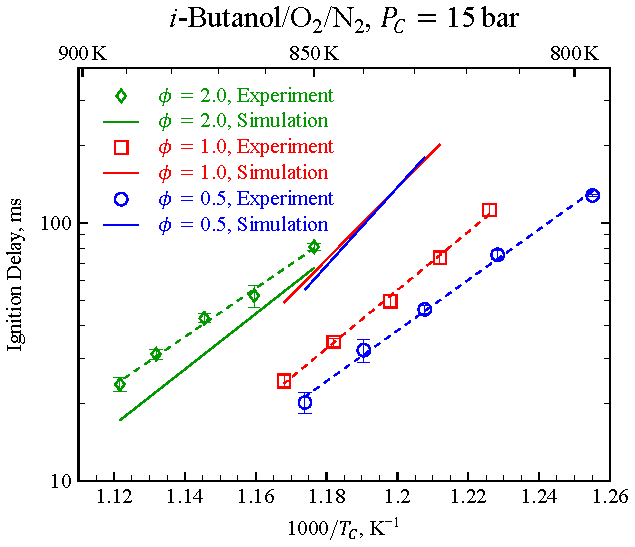
\includegraphics[width=7.9cm]{03-Butanol/ibuoh-15o2sim}}
        {\caption{Comparison of the experimentally measured ignition
        delays of \iBuOH{} at three equivalence ratios and $P_C=\SI{15}{\bar}$
        with VPRO simulations using the MIT mechanism.}
        \label{fig:ibuoh-15o2sim}}
    \ffigbox
        {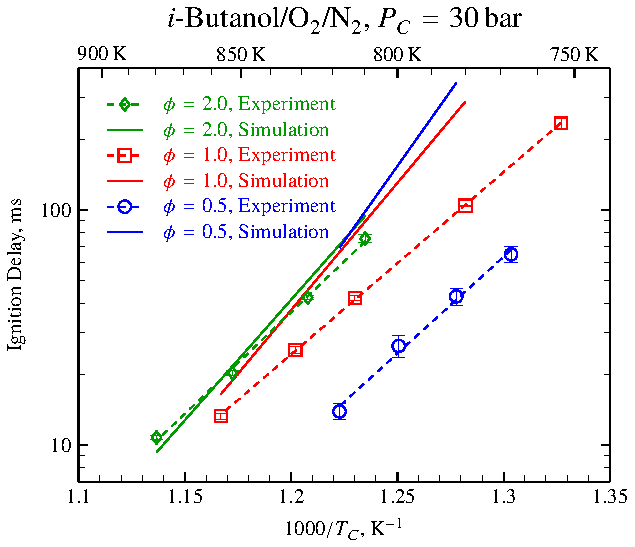
\includegraphics[width=7.9cm]{03-Butanol/ibuoh-30o2sim}}
        {\caption{Comparison of the experimentally measured ignition
        delays of \iBuOH{} at three equivalence ratios and $P_C=\SI{30}{\bar}$
        with VPRO simulations using the MIT mechanism.}
        \label{fig:ibuoh-30o2sim}}
    \end{floatrow}
\end{figure}

\section{Discussion}
\label{sec:buoh-discussion}

The relatively good agreement of the mechanism of \textcite{Sarathy2012} with
the experimental data as shown in \cref{fig:buoh-15sim,fig:buoh-30sim},
even for conditions at which the mechanism has not been
validated, suggests that using the mechanism to further interpret the
experimental data is a worthwhile exercise. In particular,
\cref{fig:buoh-npath,fig:buoh-spath,fig:buoh-tpath,fig:buoh-ipath}
show the initial steps of the fuel breakdown process for each isomer.
The percentages listed are the percent of the reactant that is consumed
to produce the product shown, by all the reactions that can produce
that product from the reactant, except where one particular reaction
is noted. These numbers are determined by integrating the
rate of production or consumption of each species by each reaction up to the
point of \SI{20}{\percent} fuel consumption, and normalizing each reaction by the total
produced or consumed of each species up to that point. The \SI{20}{\percent} fuel
consumption point is chosen because it is before small molecule chemistry takes
over to drive the ignition, and it has been used previously
\cite{Weber2011,Sarathy2012}. The rates of production are taken from a CONV
simulation, with initial conditions of \SI{750}{\kelvin} and \SI{15}{\bar} as well as \SI{750}{\kelvin} and
\SI{30}{\bar}. These conditions are representative of typical conditions after compression
in the present RCM experiments. The plain text percentages on top of the arrows
are the \SI{15}{\bar} case and the bold numbers underneath are for the \SI{30}{\bar} case.

\begin{figure}
    \begin{floatrow}
    \ffigbox
        {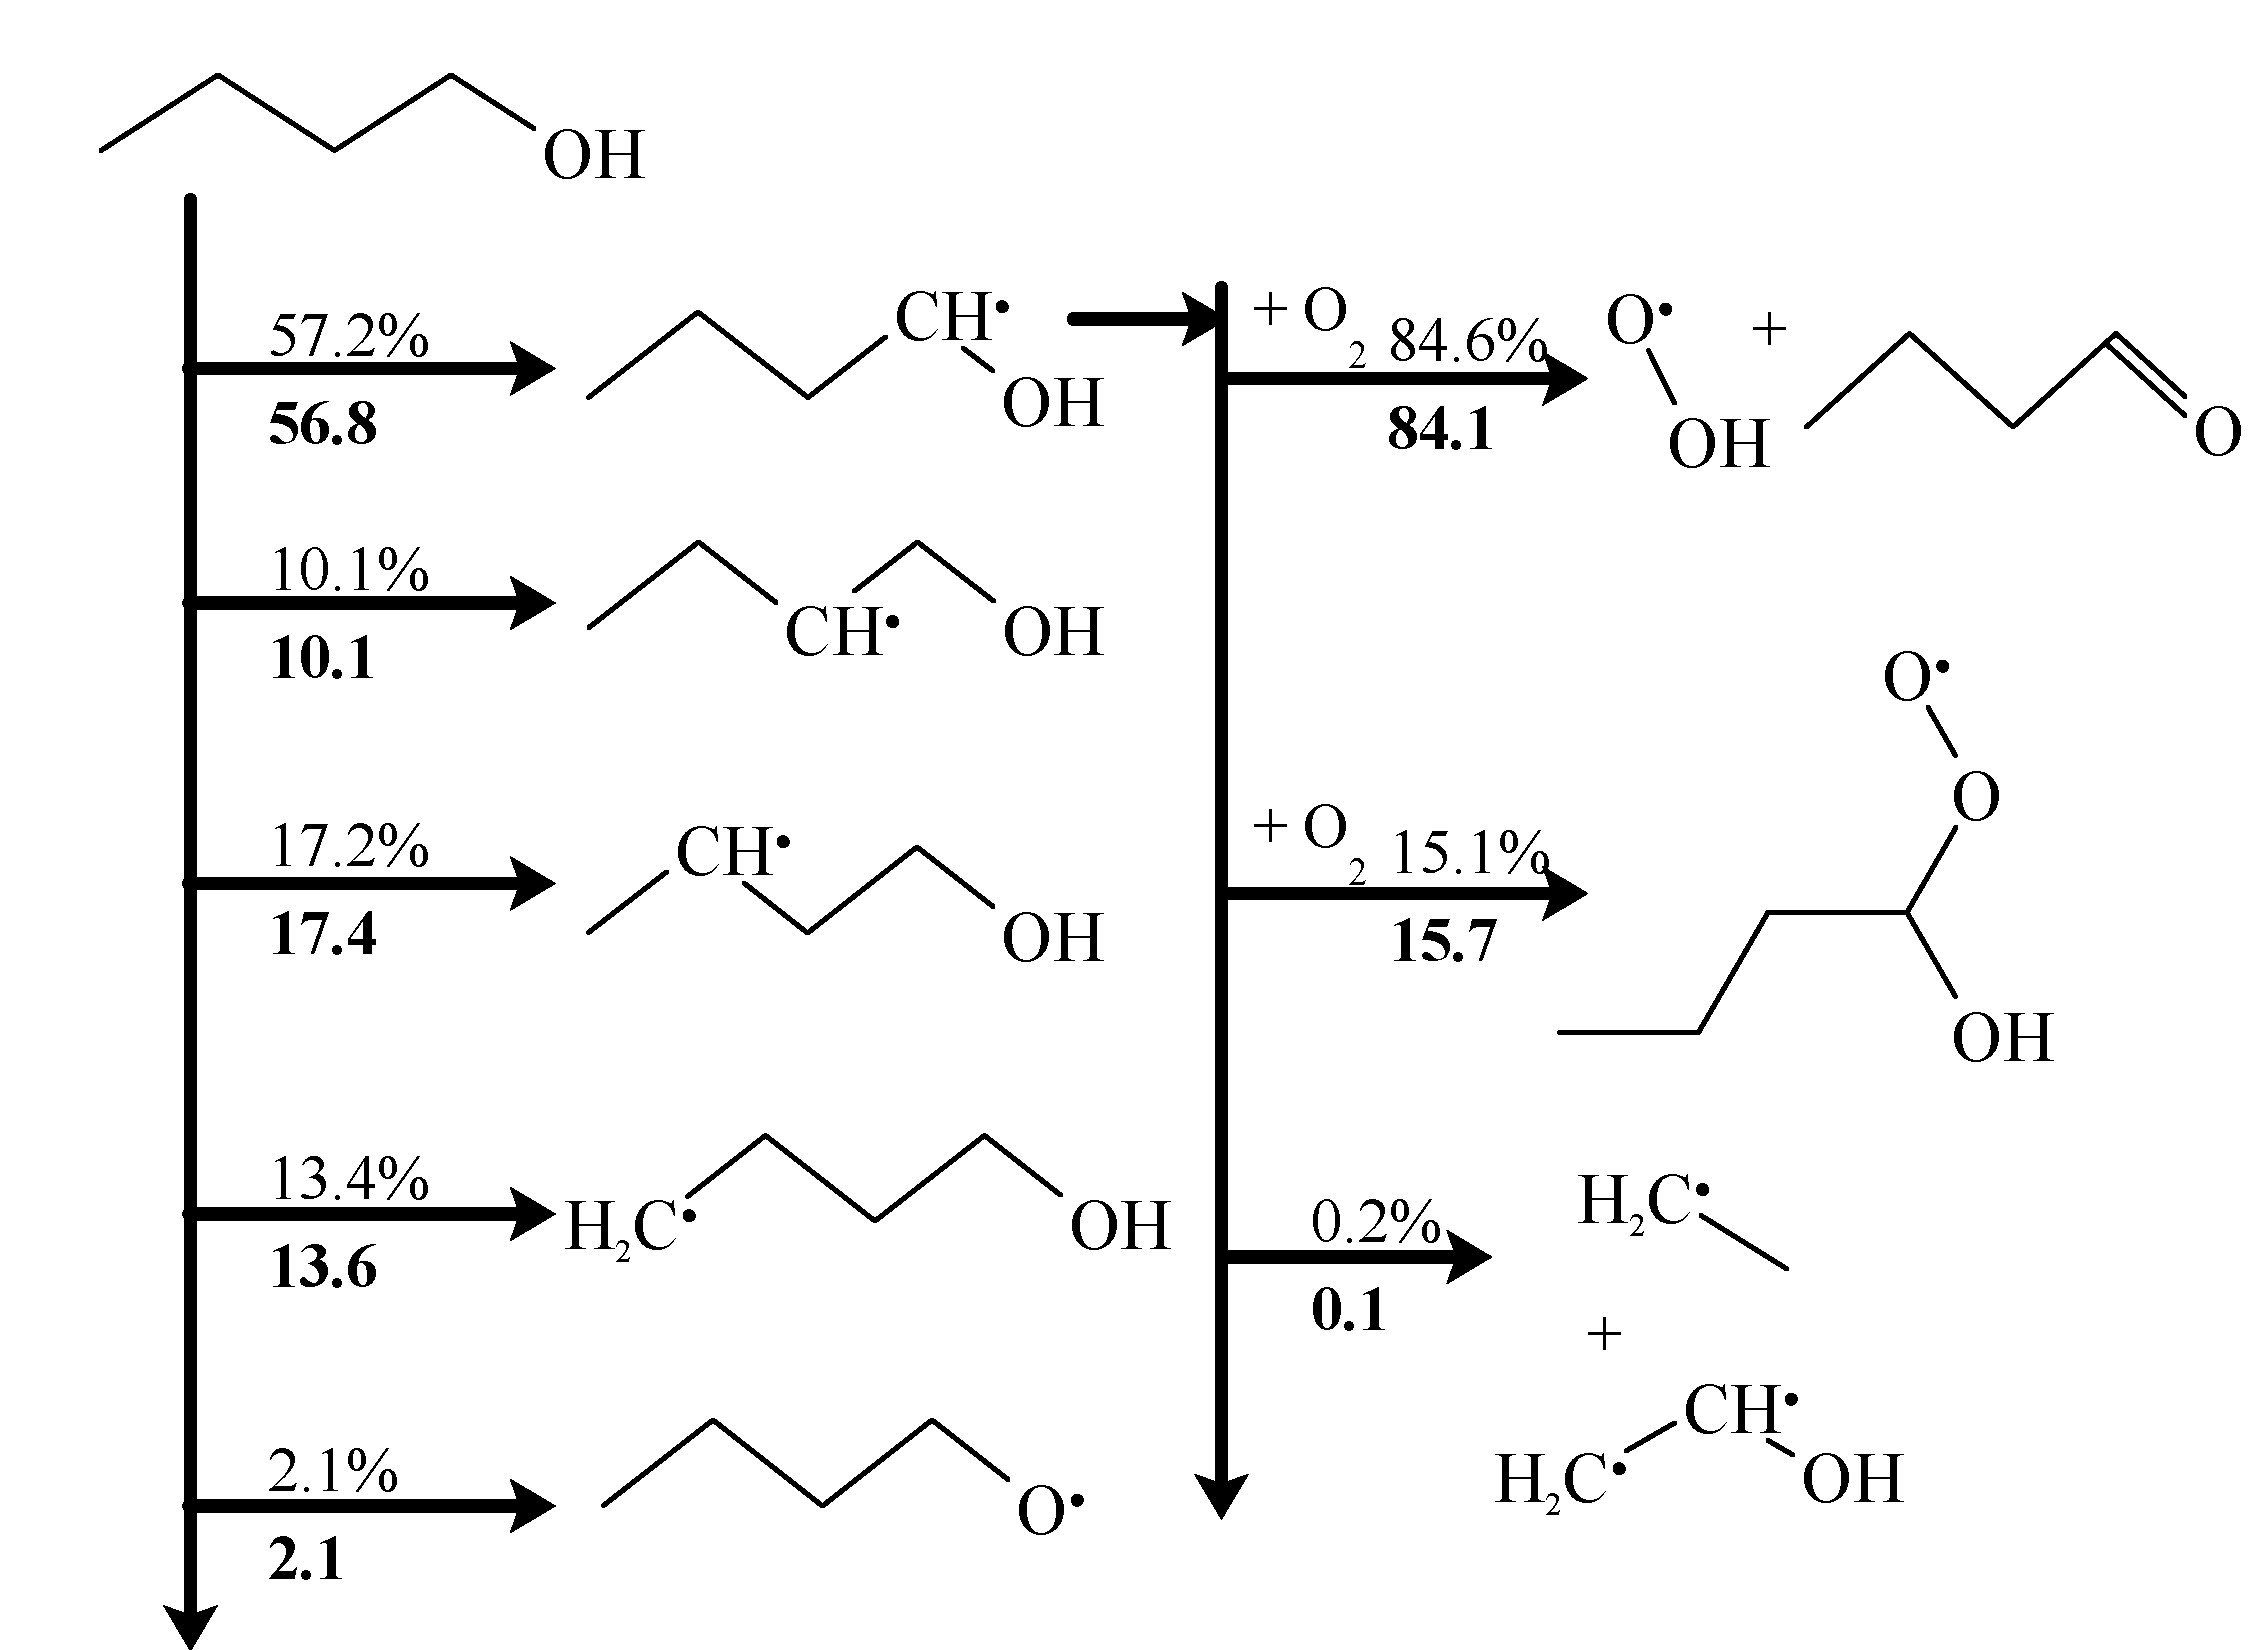
\includegraphics[width=7.9cm]{03-Butanol/buoh-npath}}
        {\caption{Pathway analysis for simulations of \nBuOH{} at
            temperature of \SI{750}{\kelvin}, in stoichiometric air, using the mechanism of
            \textcite{Sarathy2012}. Percentages in normal text represent an
            initial condition of \SI{15}{\bar}; bold text is for \SI{30}{\bar}.}
        \label{fig:buoh-npath}}
    \ffigbox
        {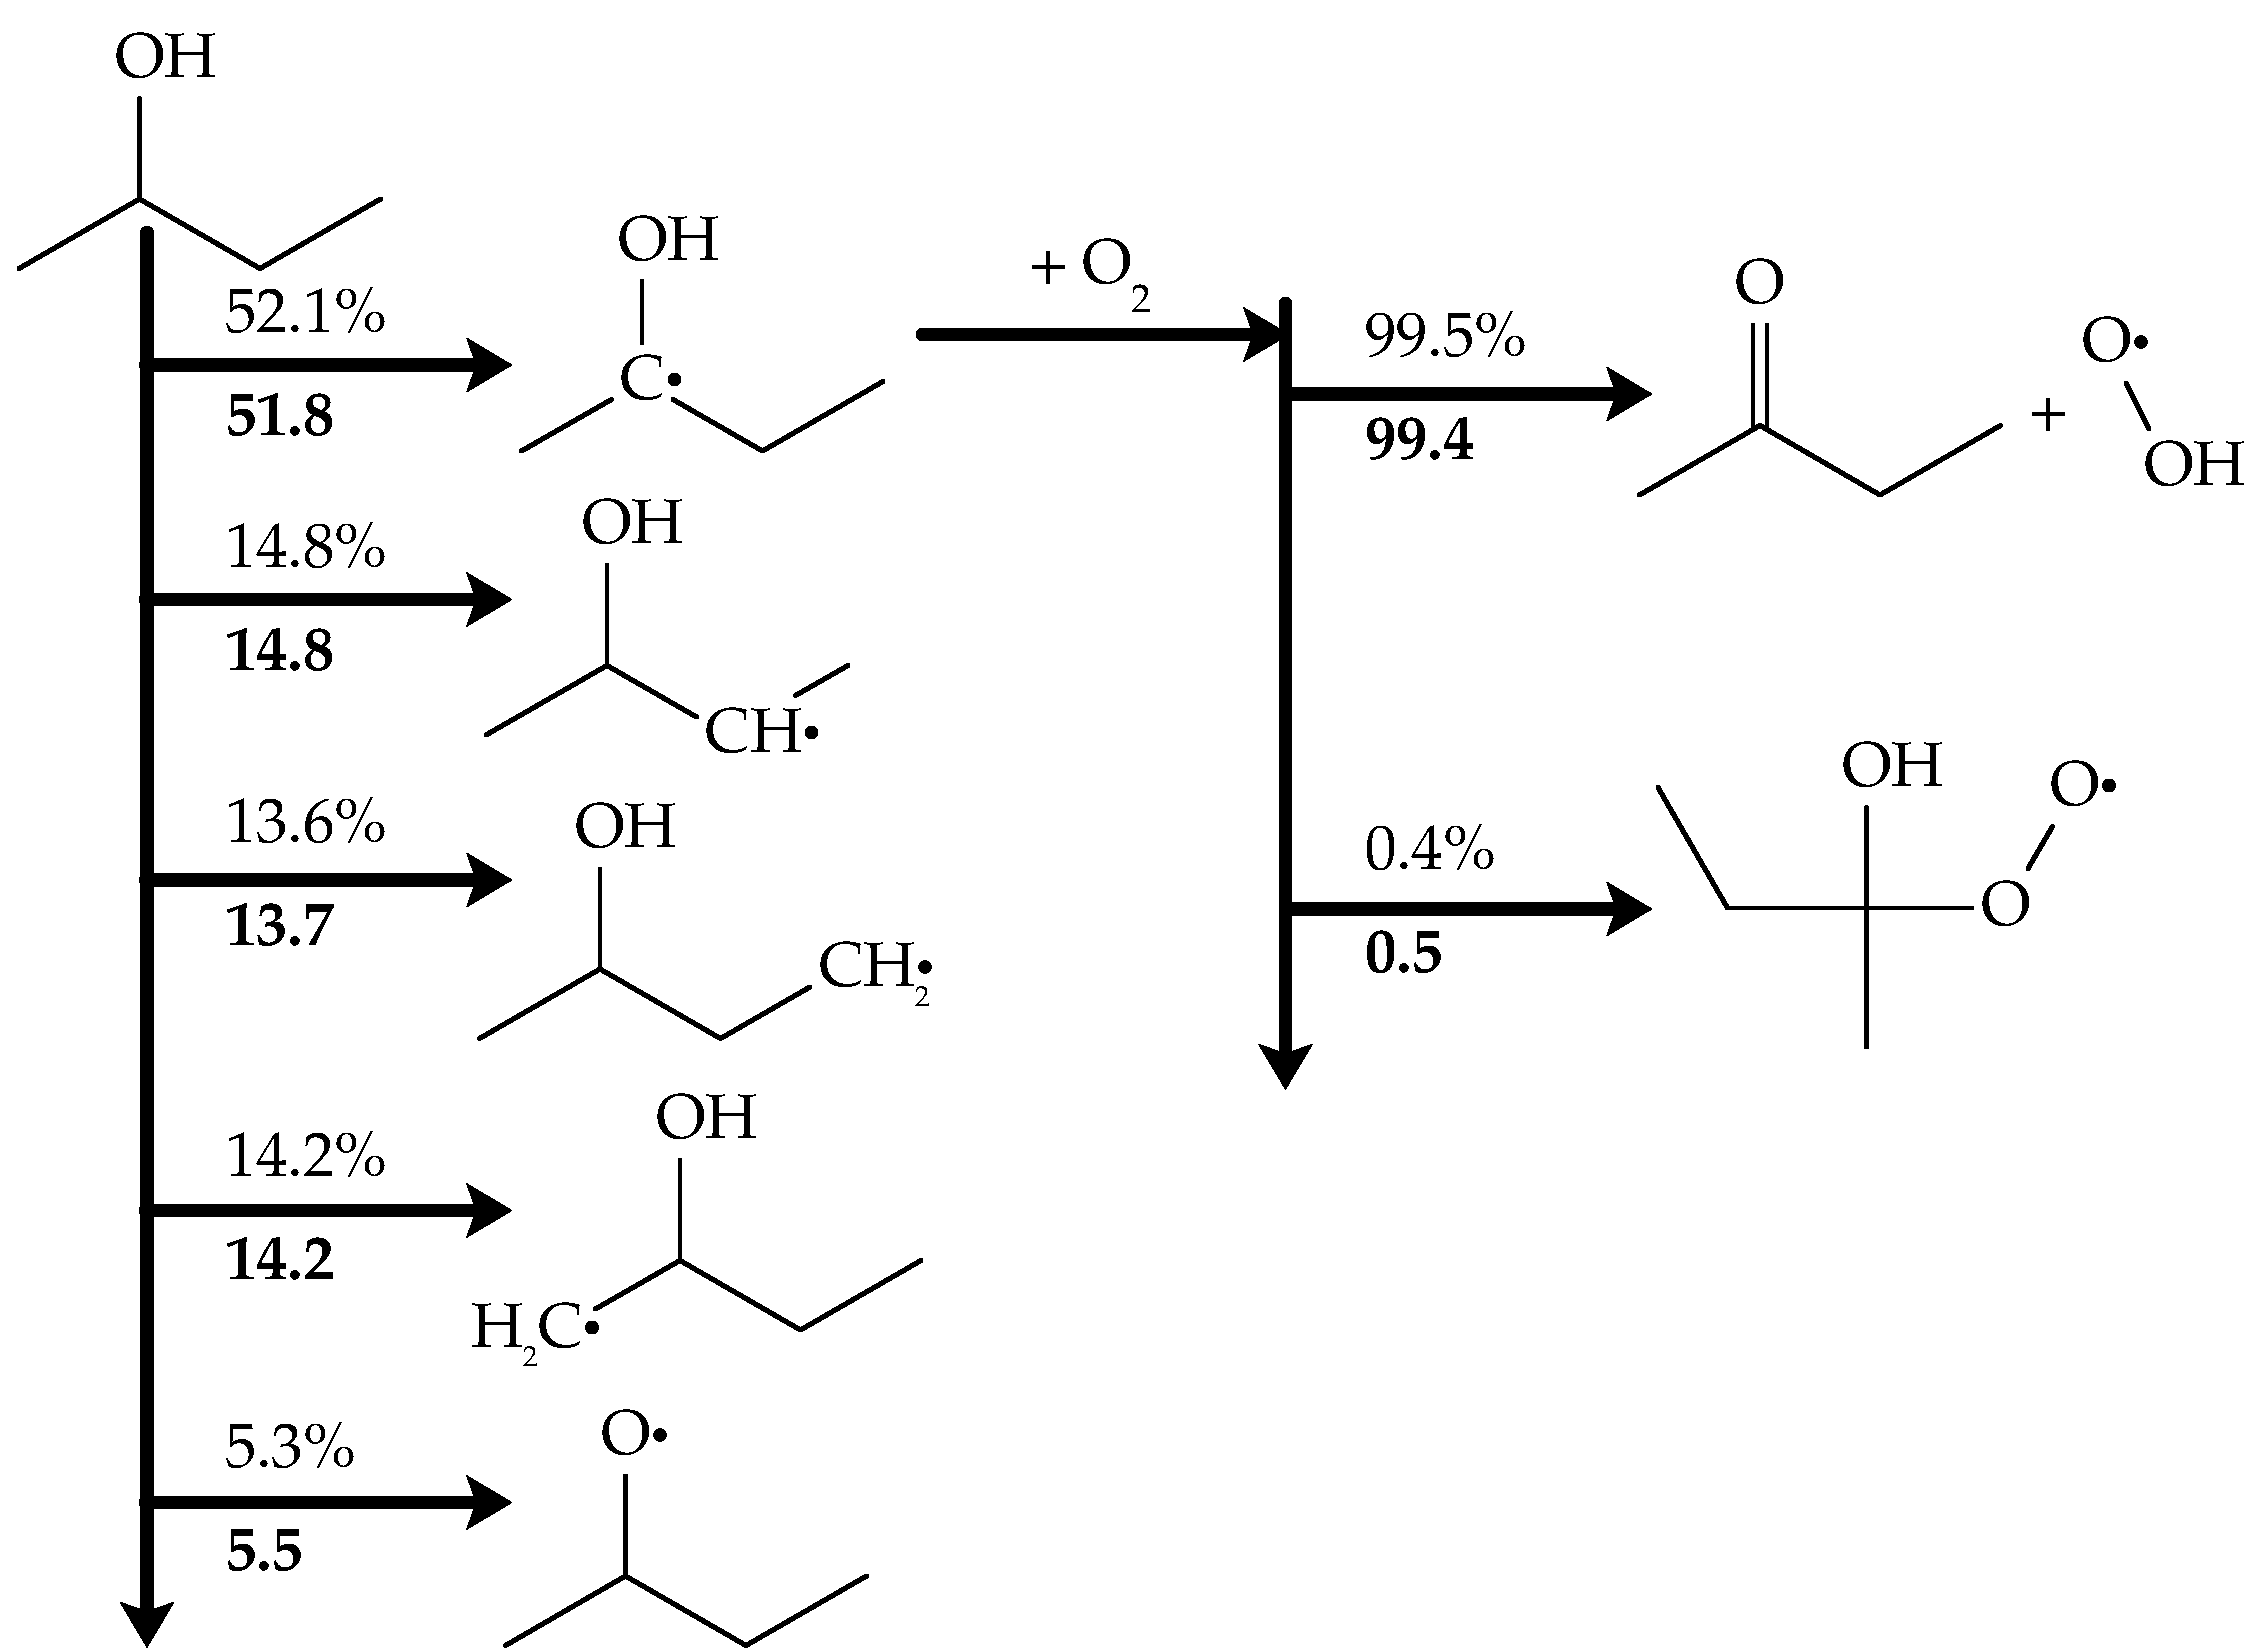
\includegraphics[width=7.9cm]{03-Butanol/buoh-spath}}
        {\caption{Pathway analysis for simulations of \sBuOH{} at
            temperature of \SI{750}{\kelvin}, in stoichiometric air, using the mechanism of
            \textcite{Sarathy2012}. Percentages in normal text represent an
            initial condition of \SI{15}{\bar}; bold text is for \SI{30}{\bar}.}
        \label{fig:buoh-spath}}
    \end{floatrow}
    \par
    \begin{floatrow}
    \ffigbox
        {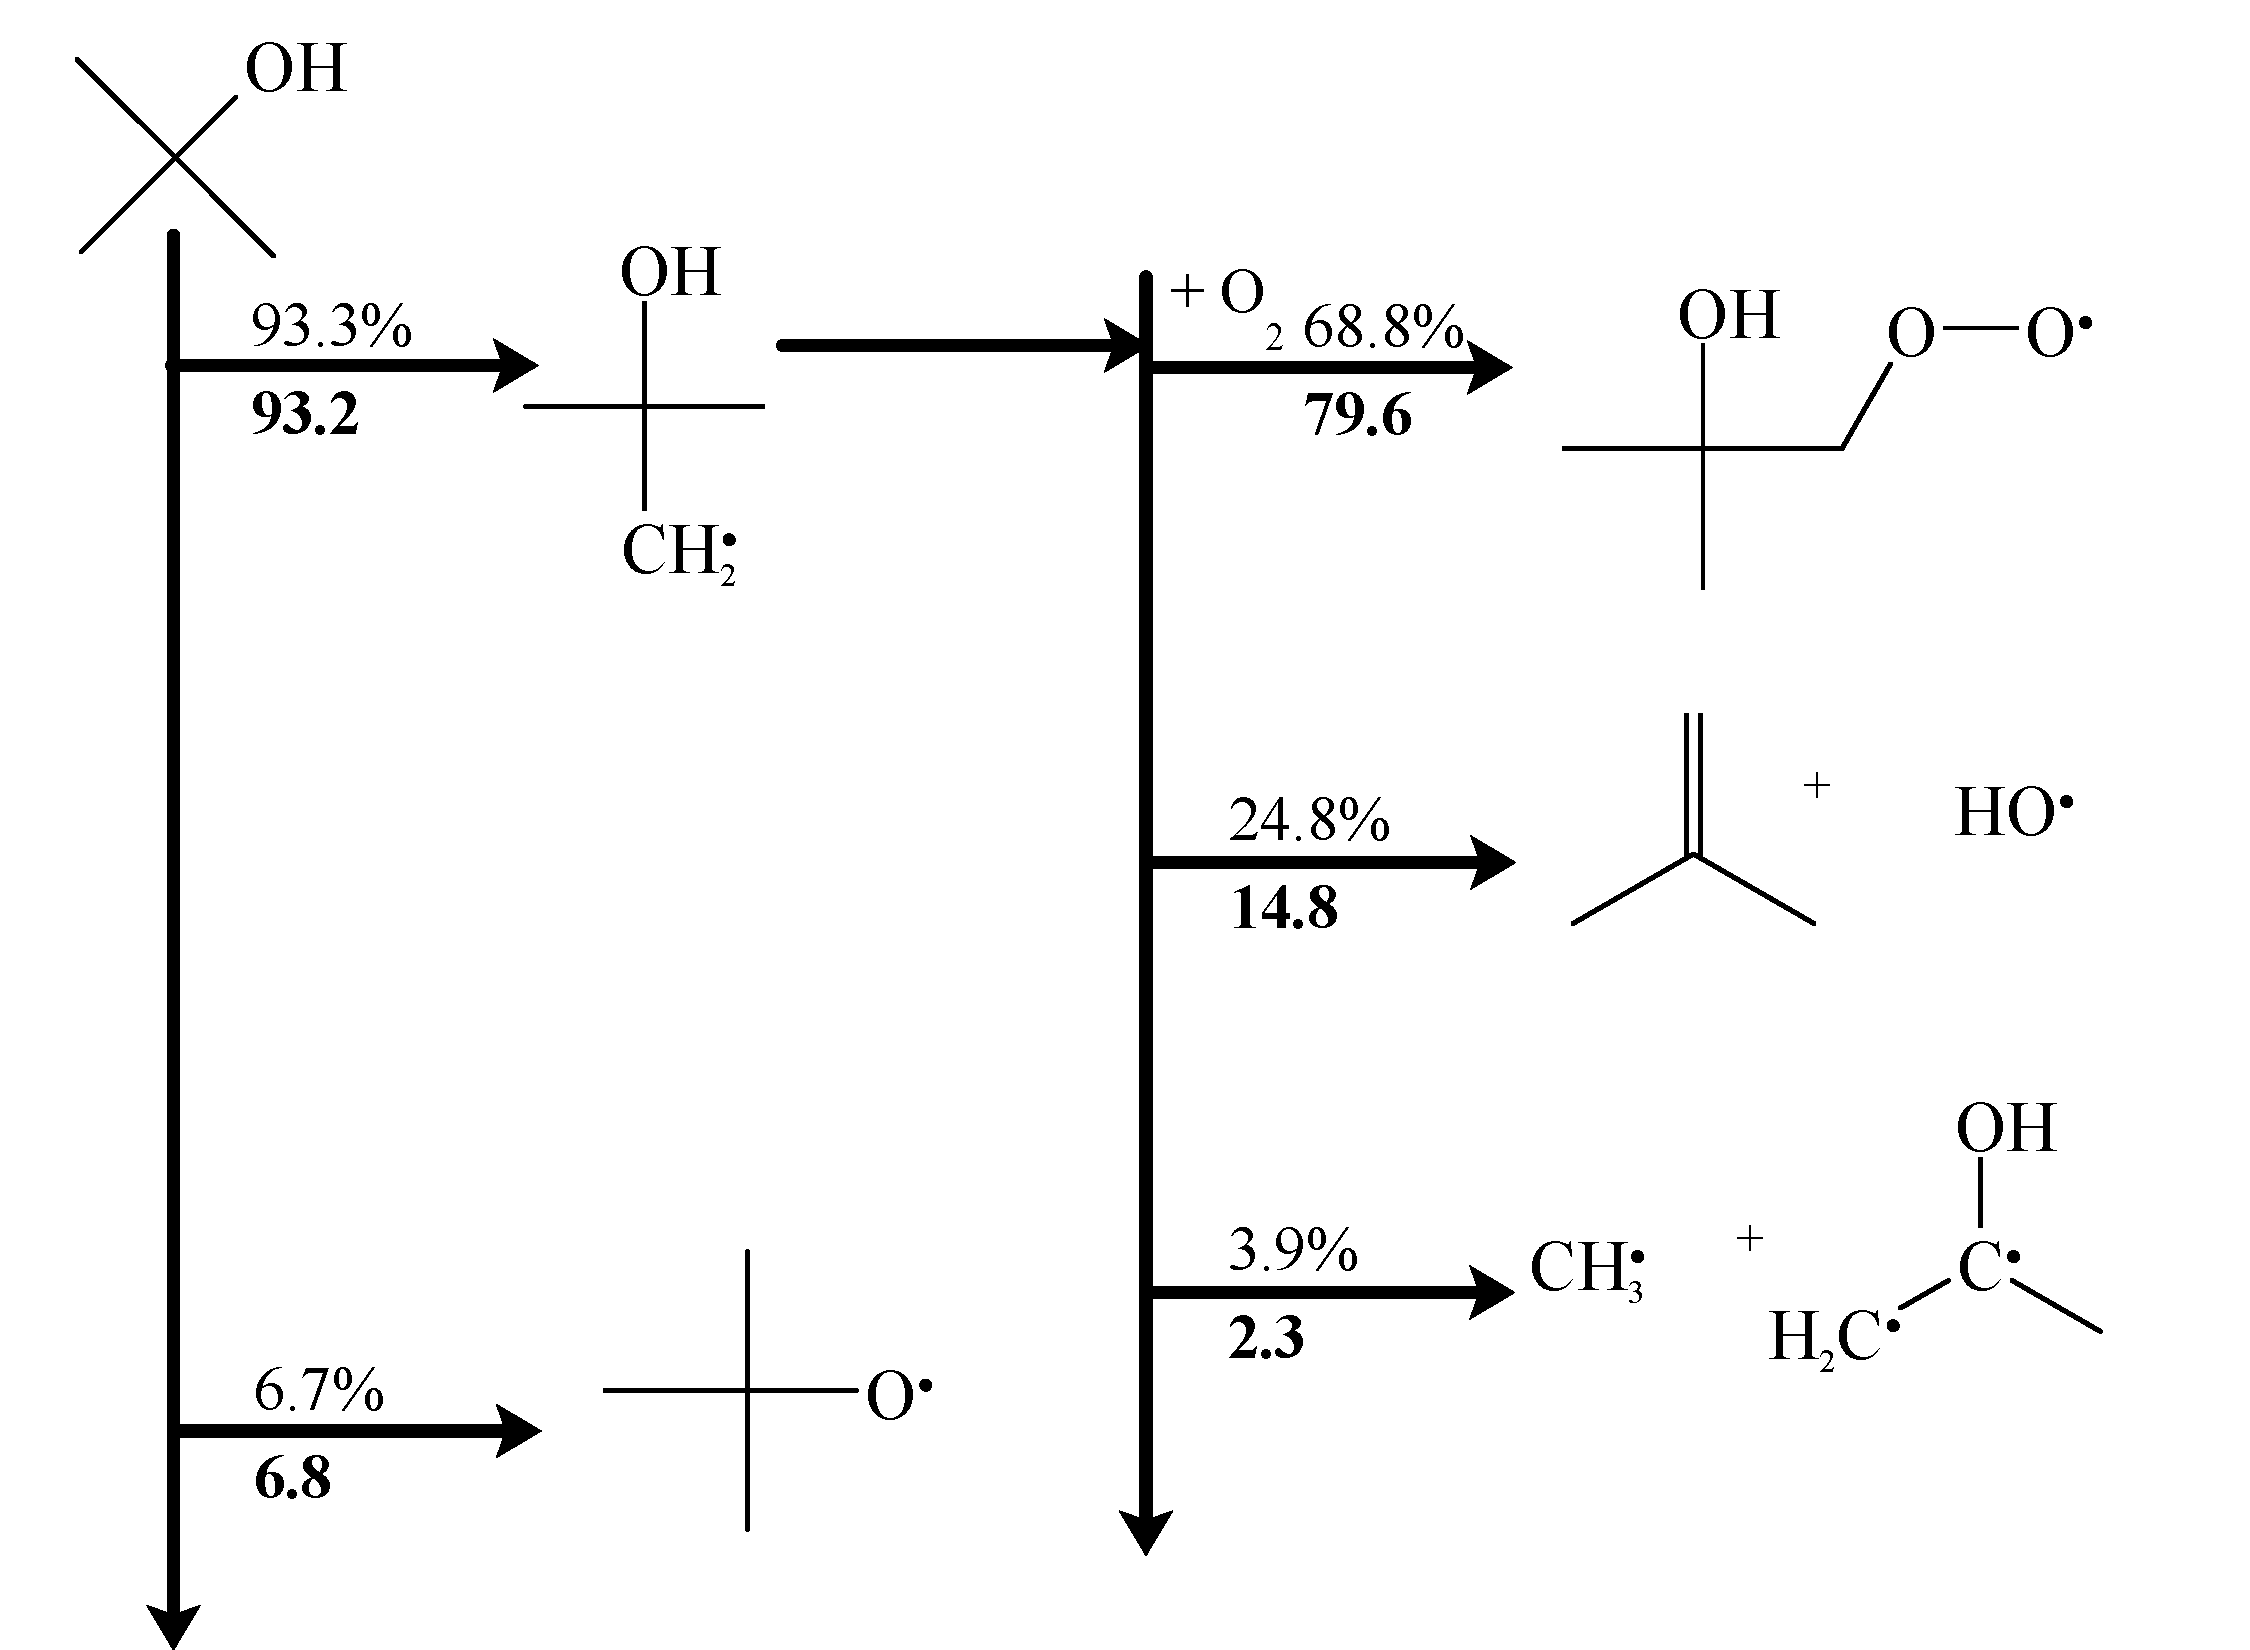
\includegraphics[width=7.9cm]{03-Butanol/buoh-tpath}}
        {\caption{Pathway analysis for simulations of \tBuOH{} at
            temperature of \SI{750}{\kelvin}, in stoichiometric air, using the mechanism of
            \textcite{Sarathy2012}. Percentages in normal text represent an
            initial condition of \SI{15}{\bar}; bold text is for \SI{30}{\bar}.}
        \label{fig:buoh-tpath}}
    \ffigbox
        {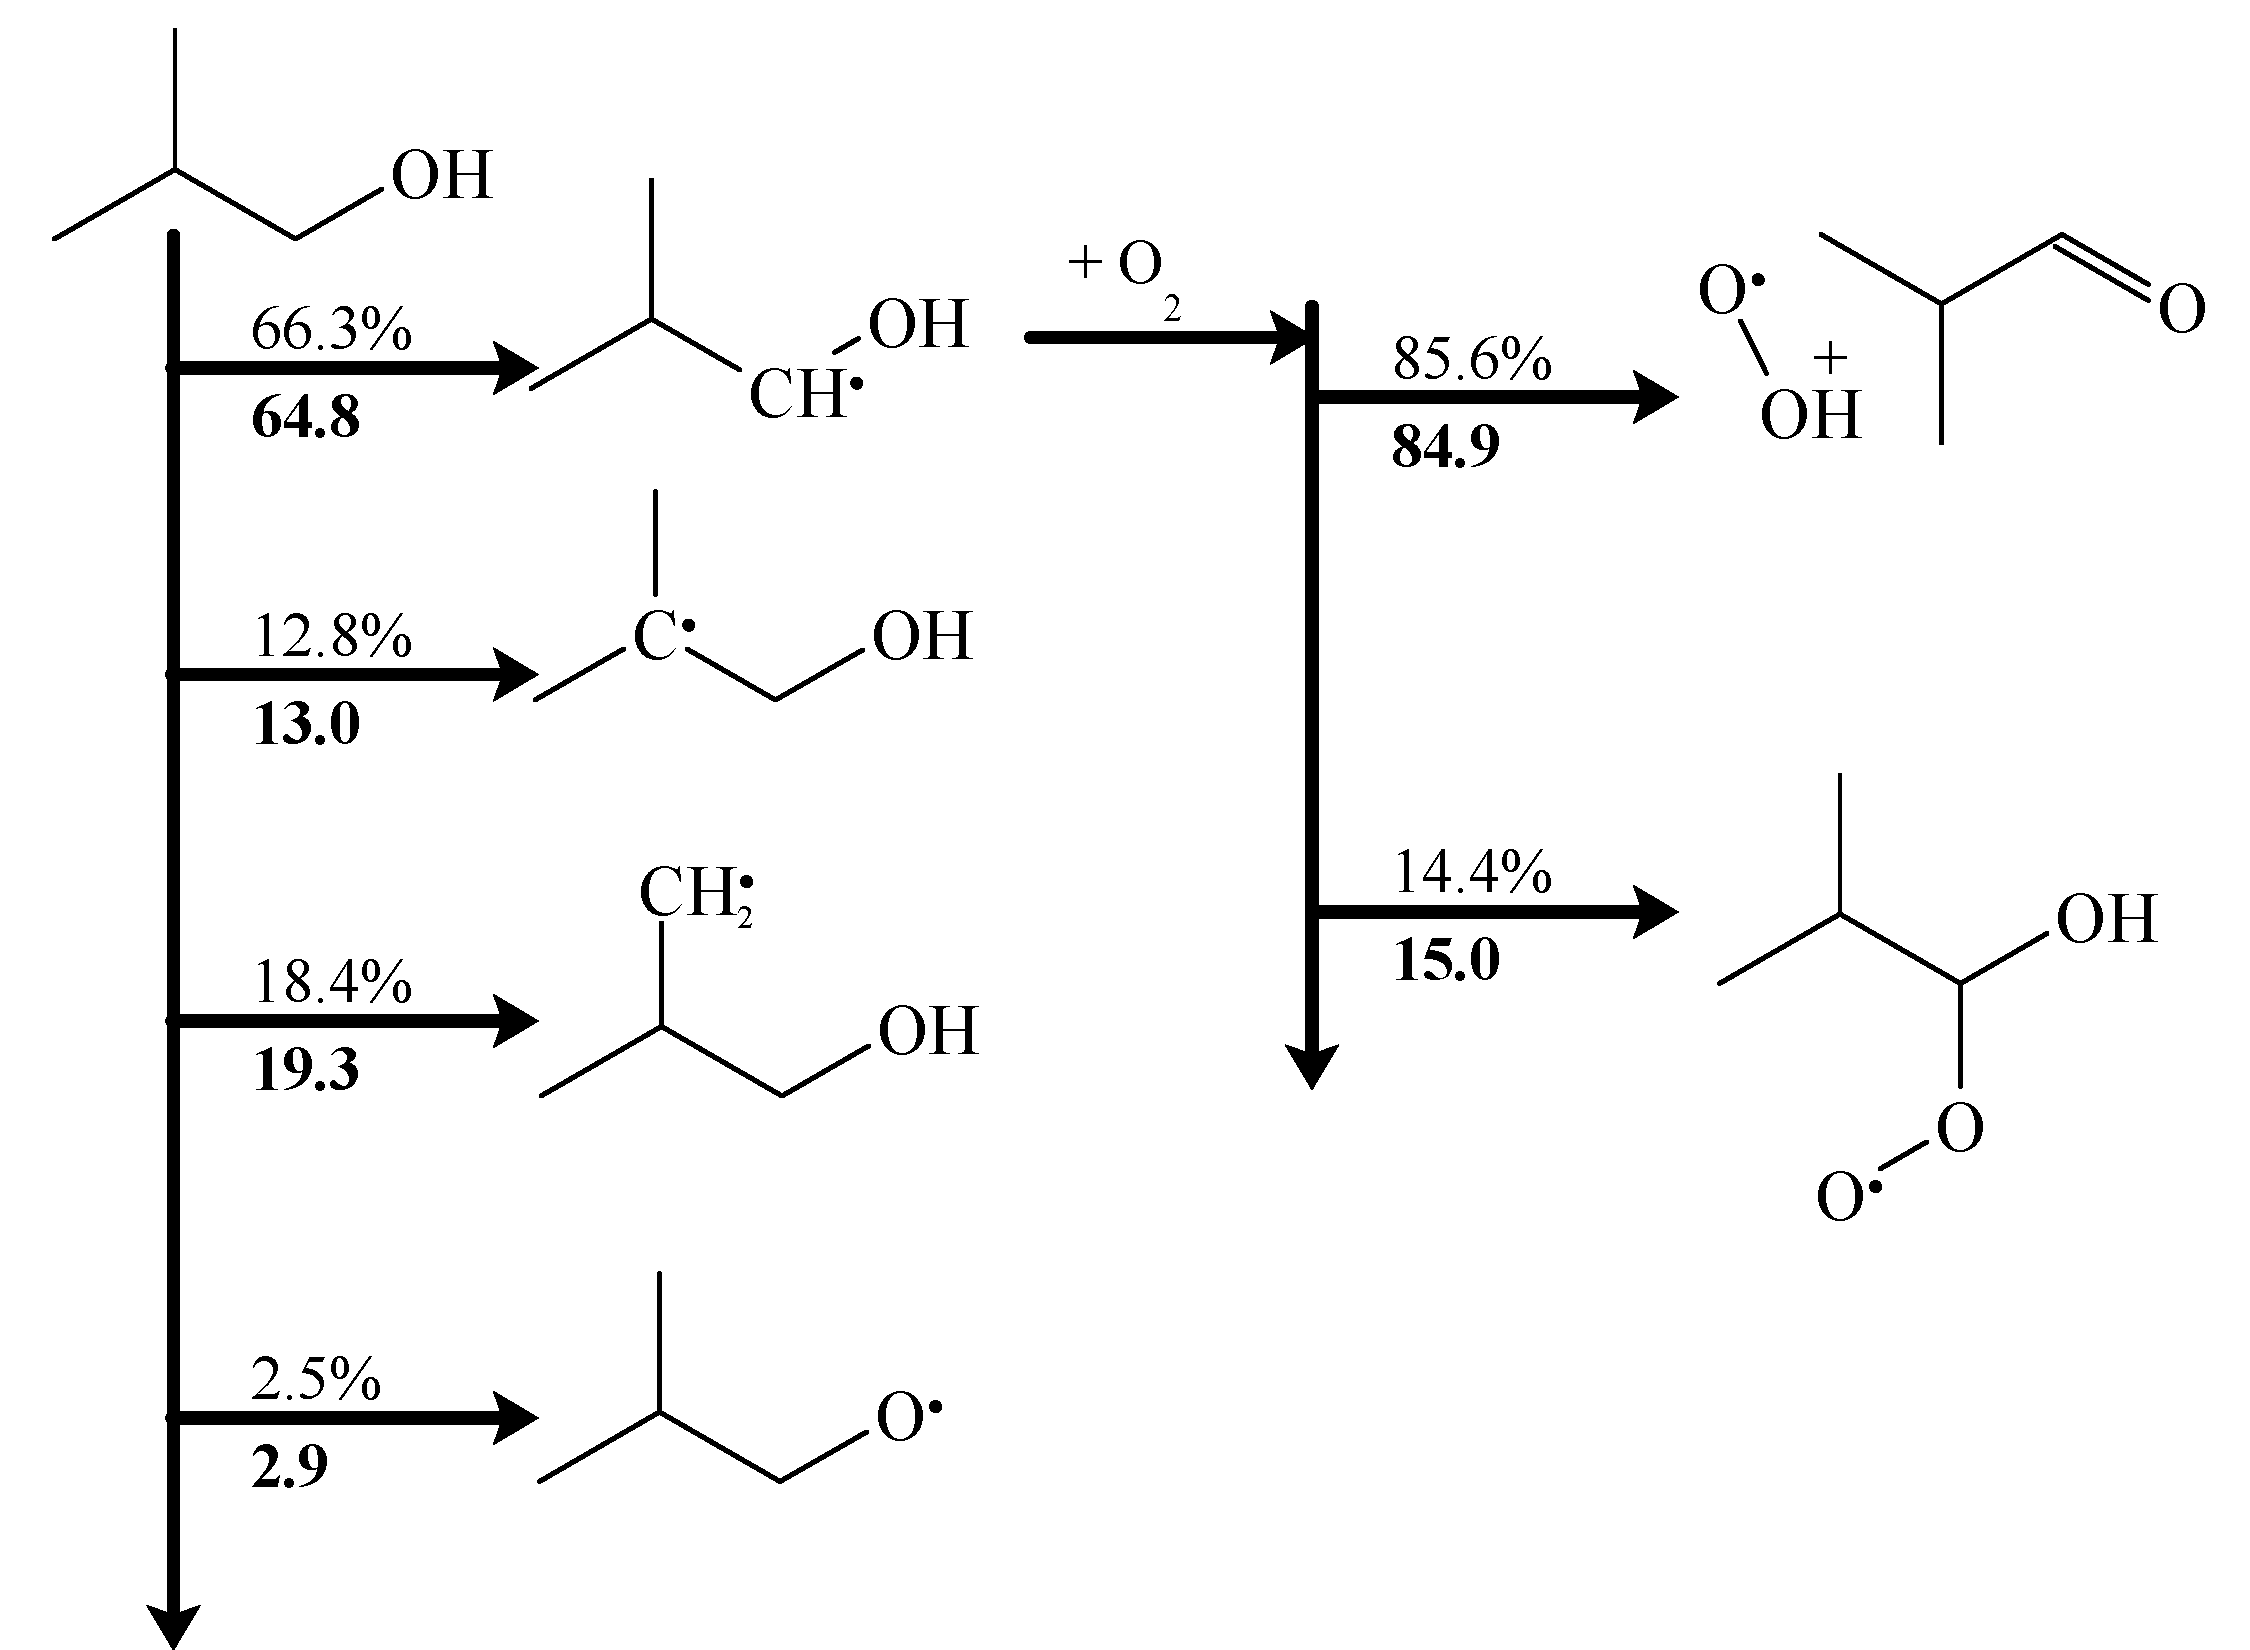
\includegraphics[width=7.9cm]{03-Butanol/buoh-ipath}}
        {\caption{Pathway analysis for simulations of \iBuOH{} at
            temperature of \SI{750}{\kelvin}, in stoichiometric air, using the mechanism of
            \textcite{Sarathy2012}. Percentages in normal text represent an
            initial condition of \SI{15}{\bar}; bold text is for \SI{30}{\bar}.}
        \label{fig:buoh-ipath}}
    \end{floatrow}
\end{figure}

In the following discussion, carbon-centered radicals are labeled according to
their distance from the hydroxyl moiety in the fuel molecule, as shown in
\cref{fig:buoh-isomers}. As expected at the relatively low temperature of this analysis, H-abstraction
reactions dominate over unimolecular decomposition for all four isomers. It is
also expected that \textit{n}-, \textit{s}-, and \iBuOH{} react
primarily to their respective $\alpha$-hydroxybutyl radicals, since the
$\alpha$ C-H bond has the lowest energy \cite{Sarathy2012}. Due to its unique
structure, \tBuOH{} does not have an $\alpha$-hydroxybutyl radical
that can be formed by H-abstraction, so \tBuOH{} is primarily
consumed to form the $\beta$-hydroxybutyl radical, because the O-H bond energy
is much higher than $\beta$ C-H bond energies.

The unique structure of \tBuOH{} continues to affect the second level
of reactions. In the temperature and pressure regime investigated,
\tBuOH{} tends to add to molecular oxygen at the carbon radical site,
forming a hydroxybutylperoxy (RO$_2$) species. That this pathway is dominant is
due to the fact that \tBuOH{} has no $\alpha$-hydroxybutyl radical.
For the other three butanol isomers that do have an $\alpha$-hydroxybutyl
radical, the second level of reactions primarily produces an aldehyde + HO$_2$
by direct reaction–--no hydroxybutylperoxy adduct is formed in this reaction,
and there is no possibility for typical hydrocarbon low-temperature chain
branching. Therefore, it is hypothesized that the pre-ignition heat release
seen in \tBuOH{} is caused by the oxygen addition to the fuel radical
to form $\beta$-hydroxybutylperoxy, which is an exothermic reaction.

\Cref{fig:buoh-heat} shows the total cumulative heat release of each isomer
and the cumulative heat release of an important reaction for each of the
isomers (inset), from a CONV simulation with initial conditions of \SI{750}{\kelvin} and
\SI{30}{\bar}; analysis of \SI{15}{\bar} results is substantially similar. The cumulative heat
release in the inset is found by integrating the heat release by each reaction
with respect to time, while the reactions shown are the respective reactions
that have released the most heat up to the \SI{20}{\percent} fuel consumption point for each
isomer. The abscissa of the plot is the fuel conversion, in percent. This
choice of x-axis allows a fair comparison of the heat release, because the
ignition delays of each isomer are markedly different, so comparing the heat
release with a time axis is more difficult. In \cref{fig:buoh-heat},
exothermicity is represented by positive quantities.

In \cref{fig:buoh-heat}, it is clear that \tBuOH{} has higher
heat release at low fuel consumption (during the induction period) than the
other three isomers. In addition, the primary heat release reaction for
\tBuOH{} has created much more heat than the primary reactions of the
other three isomers. As the reactions proceed, and the temperature increases,
the reverse reaction in the \tBuOH{} case becomes more important, and
the heat release contribution of this oxygen-addition reaction levels off. The
dominance of this reaction at early times is unique to \tBuOH{}
ignition, and appears to be driving the pre-ignition heat release.

\begin{figure}
    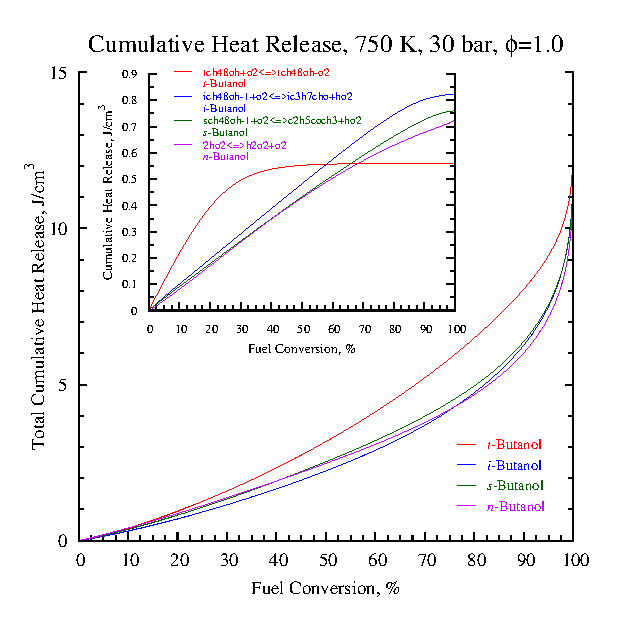
\includegraphics[height=11cm]{03-Butanol/buoh-heat}
    \caption{Total cumulative heat release and cumulative heat release by
        important reactions (inset) as a function of fuel consumption from a
        simulation using the mechanism of \textcite{Sarathy2012} with initial
        conditions of \SI{750}{\kelvin} and \SI{30}{\bar}, in stoichiometric air. See
        \cref{fig:buoh-reacs} for definitions of reactions in the inset.}
    \label{fig:buoh-heat}
\end{figure}

\begin{figure}
    R1: \quad \raisebox{-0.5\height}{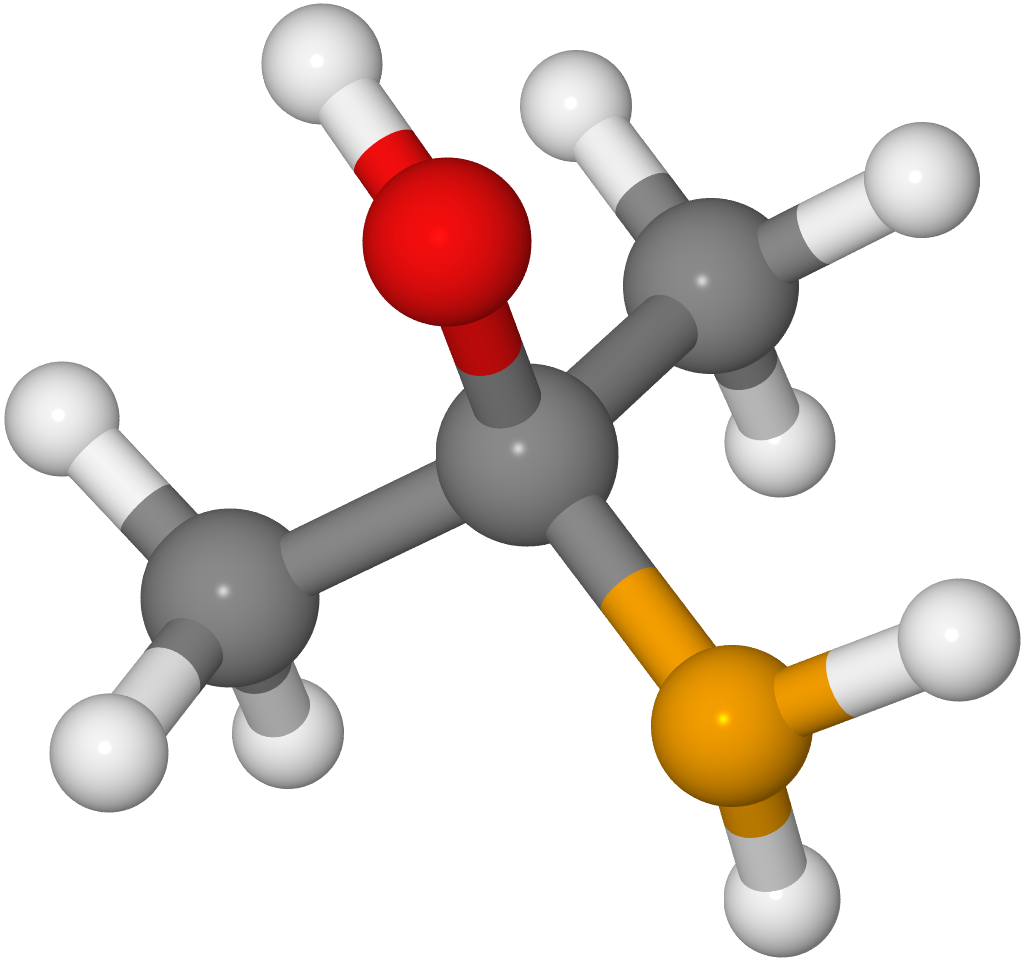
\includegraphics[height=2cm]{03-Butanol/buoh-reactions/tc4h8oh}}
    {\Large \textbf{+}}\enspace
    \raisebox{-0.5\height}{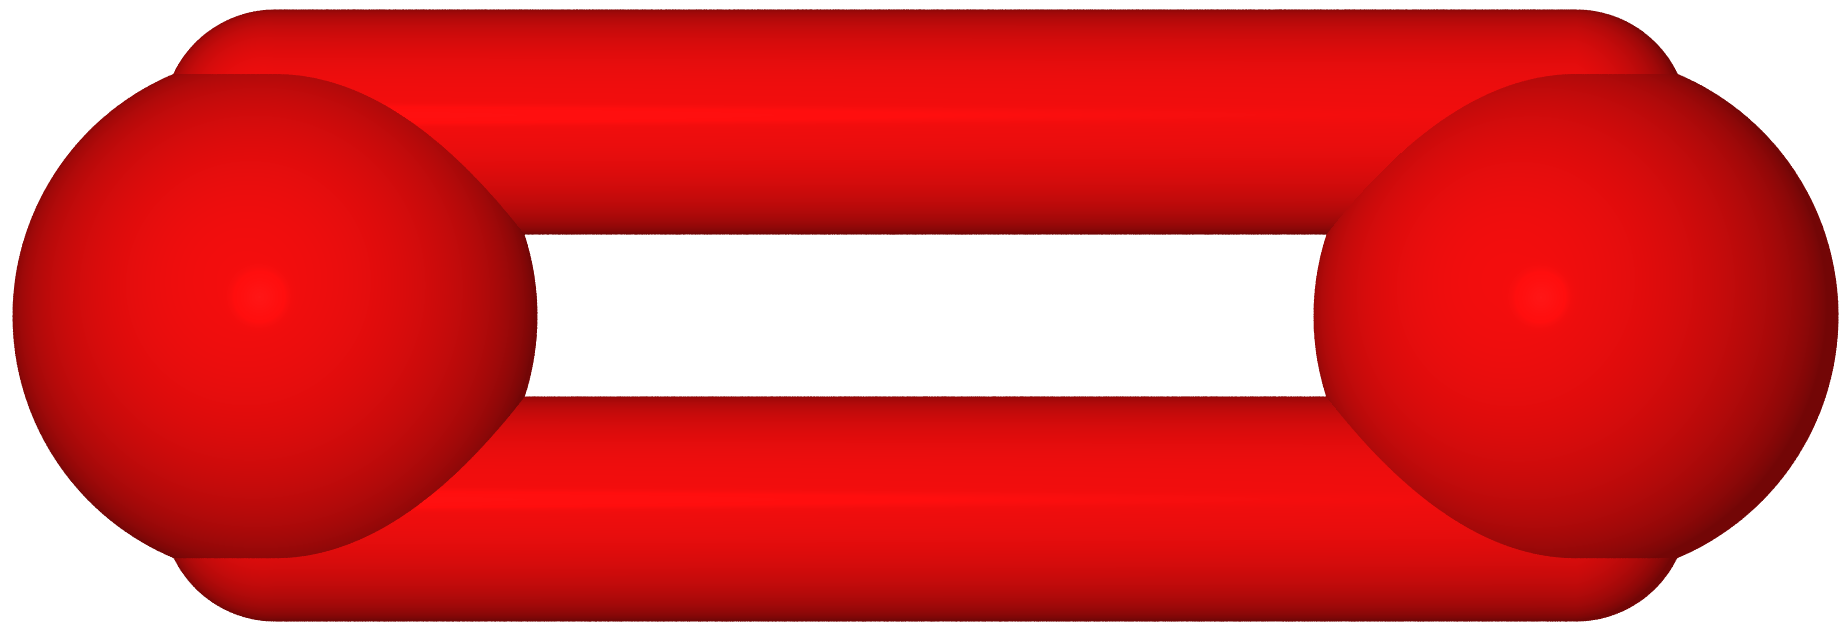
\includegraphics[height=0.5cm]{03-Butanol/buoh-reactions/oxygen}}
    {\Large \textbf{$\leftrightarrow$}}
    \raisebox{-0.5\height}{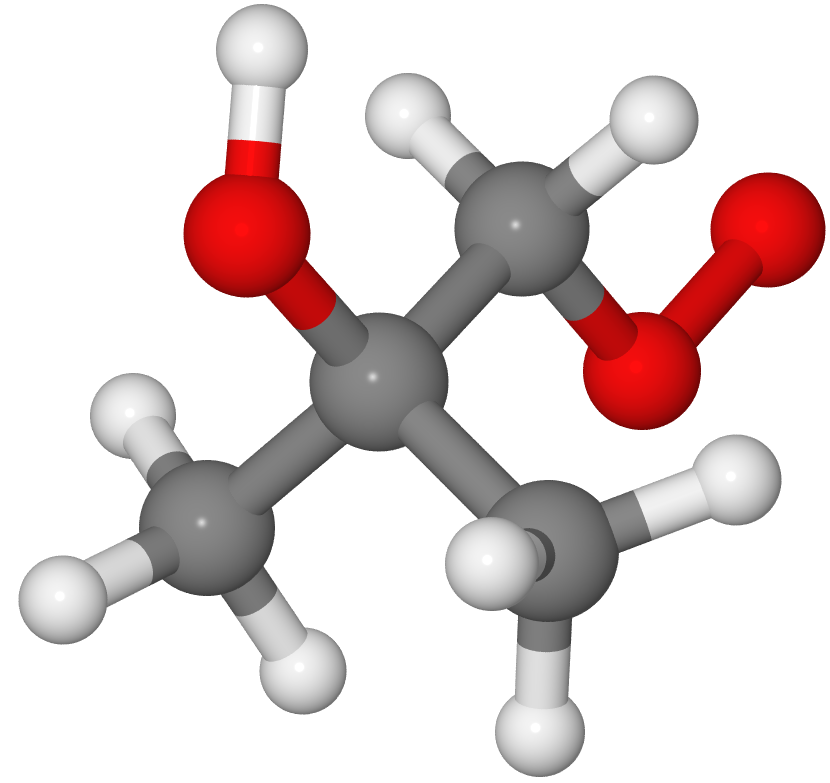
\includegraphics[height=2cm]{03-Butanol/buoh-reactions/t-hydroxybutylperoxy}}

    R2: \quad \raisebox{-0.5\height}{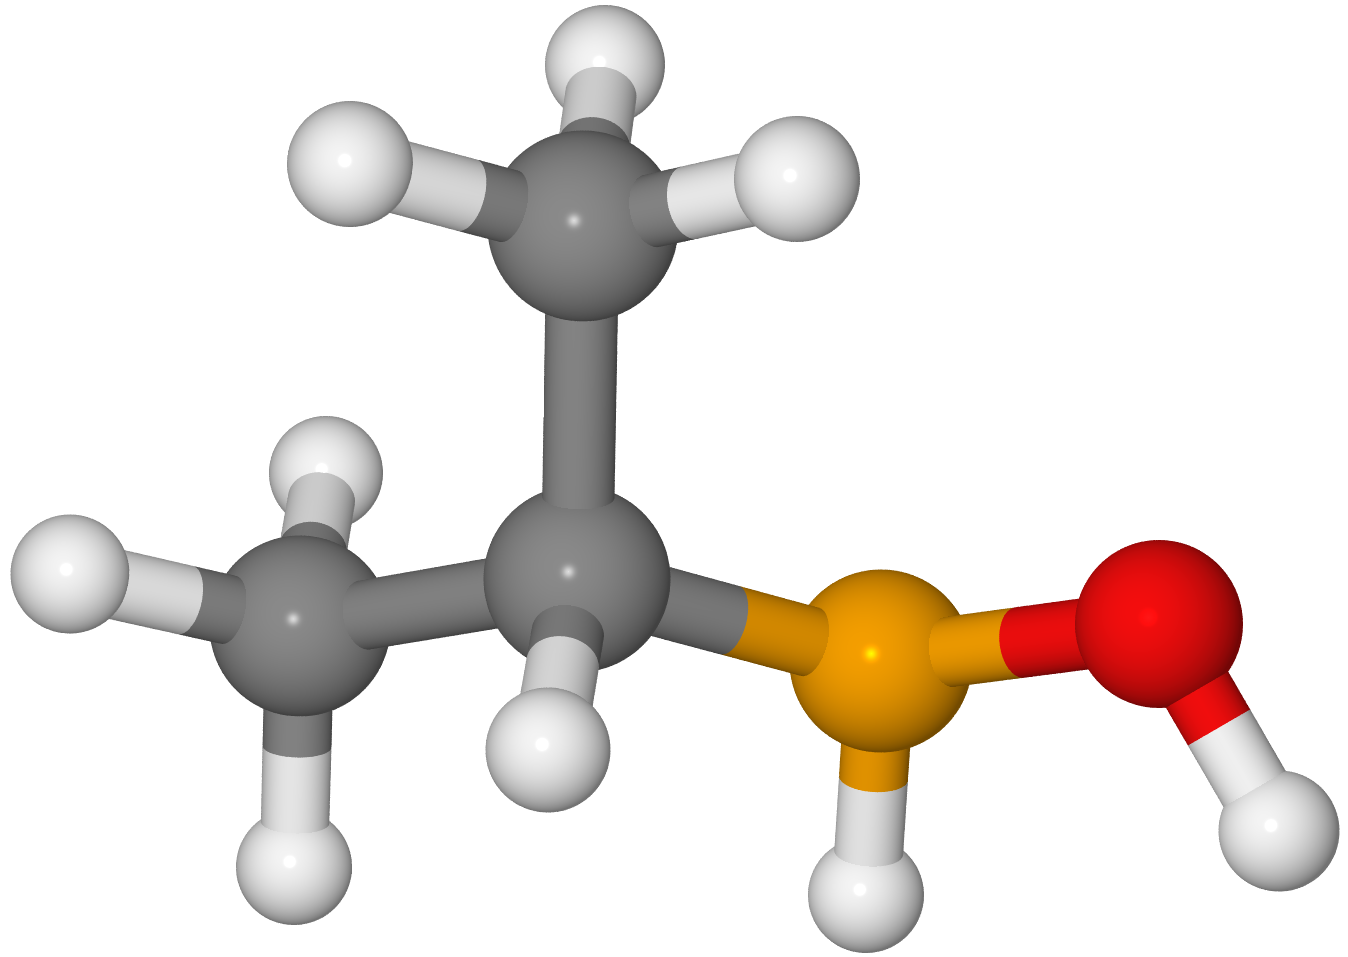
\includegraphics[height=2cm]{03-Butanol/buoh-reactions/ic4h8oh-1}}
    {\Large \textbf{+}}\enspace
    \raisebox{-0.5\height}{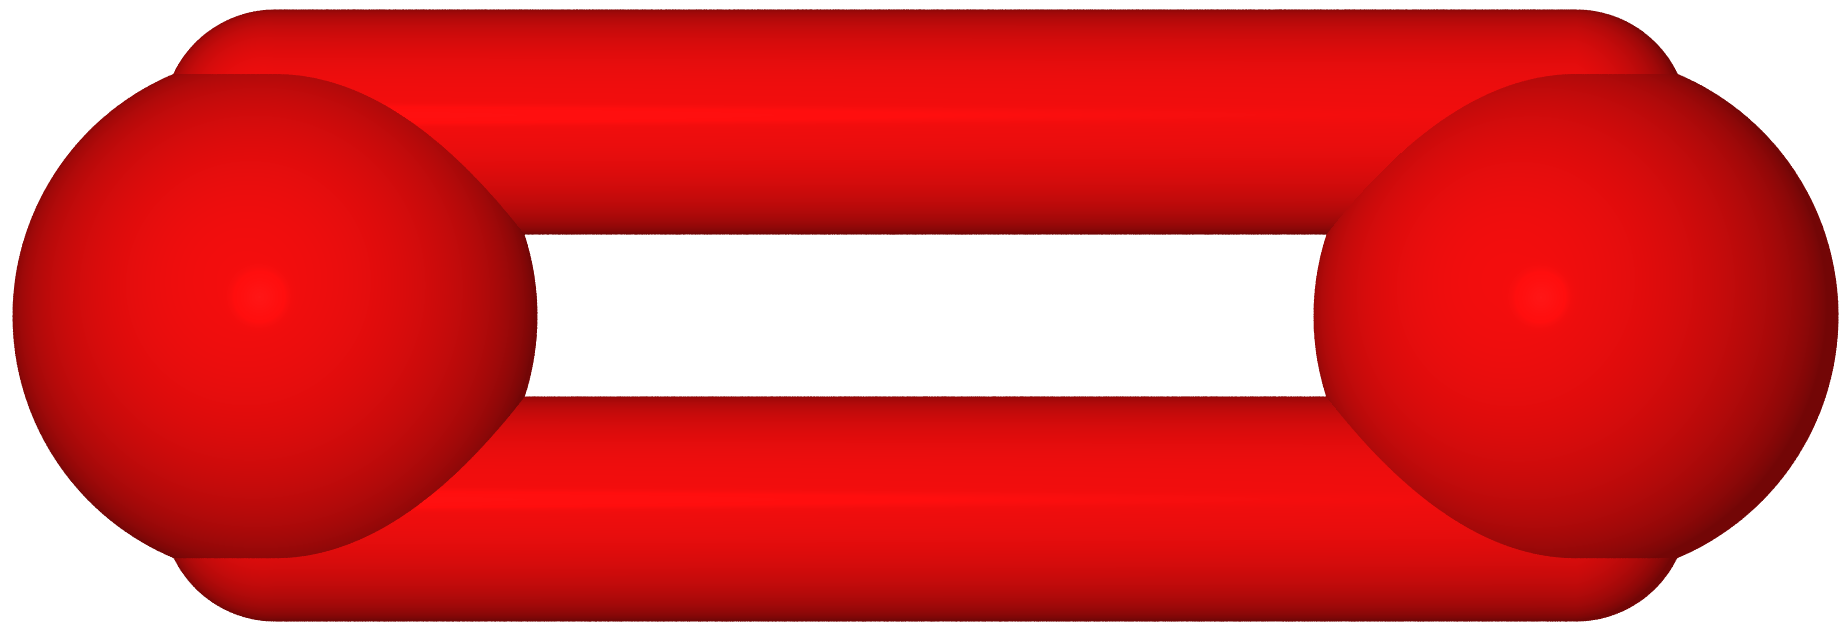
\includegraphics[height=0.5cm]{03-Butanol/buoh-reactions/oxygen}}
    \enspace{\Large \textbf{$\leftrightarrow$}}
    \raisebox{-0.5\height}{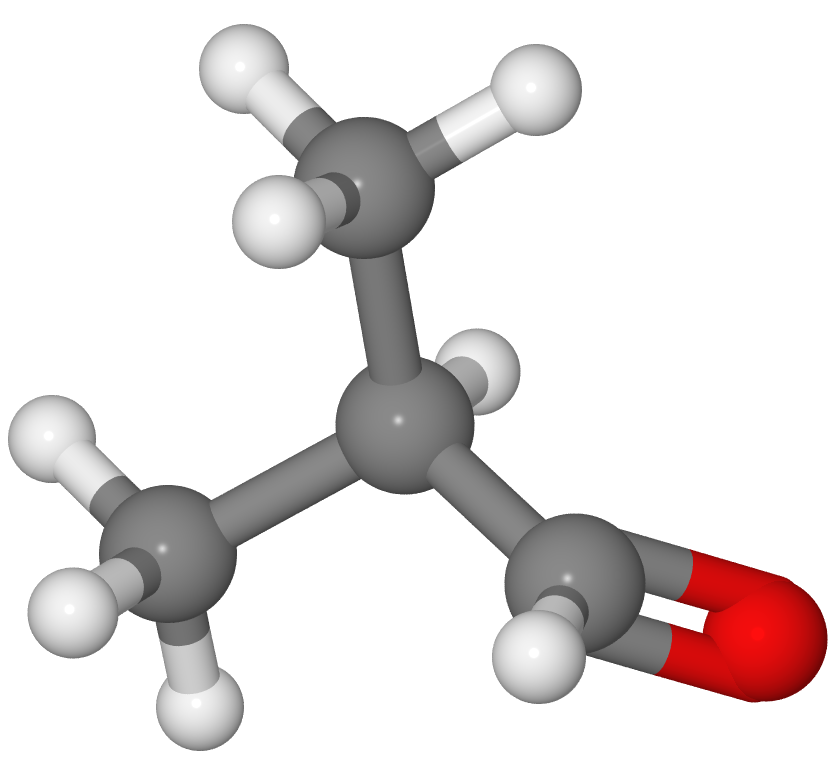
\includegraphics[height=2cm]{03-Butanol/buoh-reactions/iso-butanal}}
    {\Large \textbf{+}}\enspace
    \raisebox{-0.5\height}{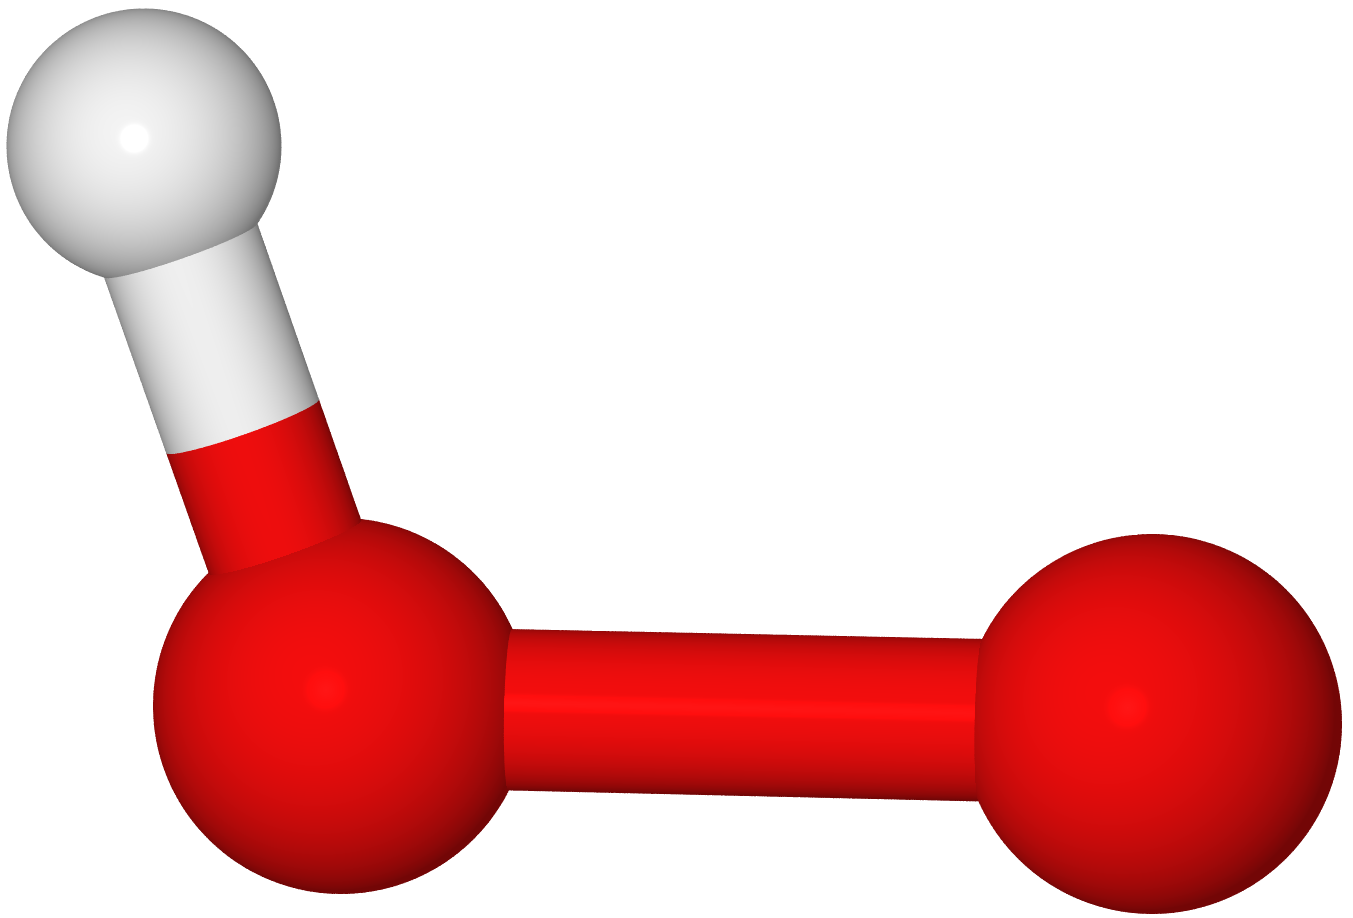
\includegraphics[height=1cm]{03-Butanol/buoh-reactions/hydroperoxy}}

    R3: \quad \raisebox{-0.5\height}{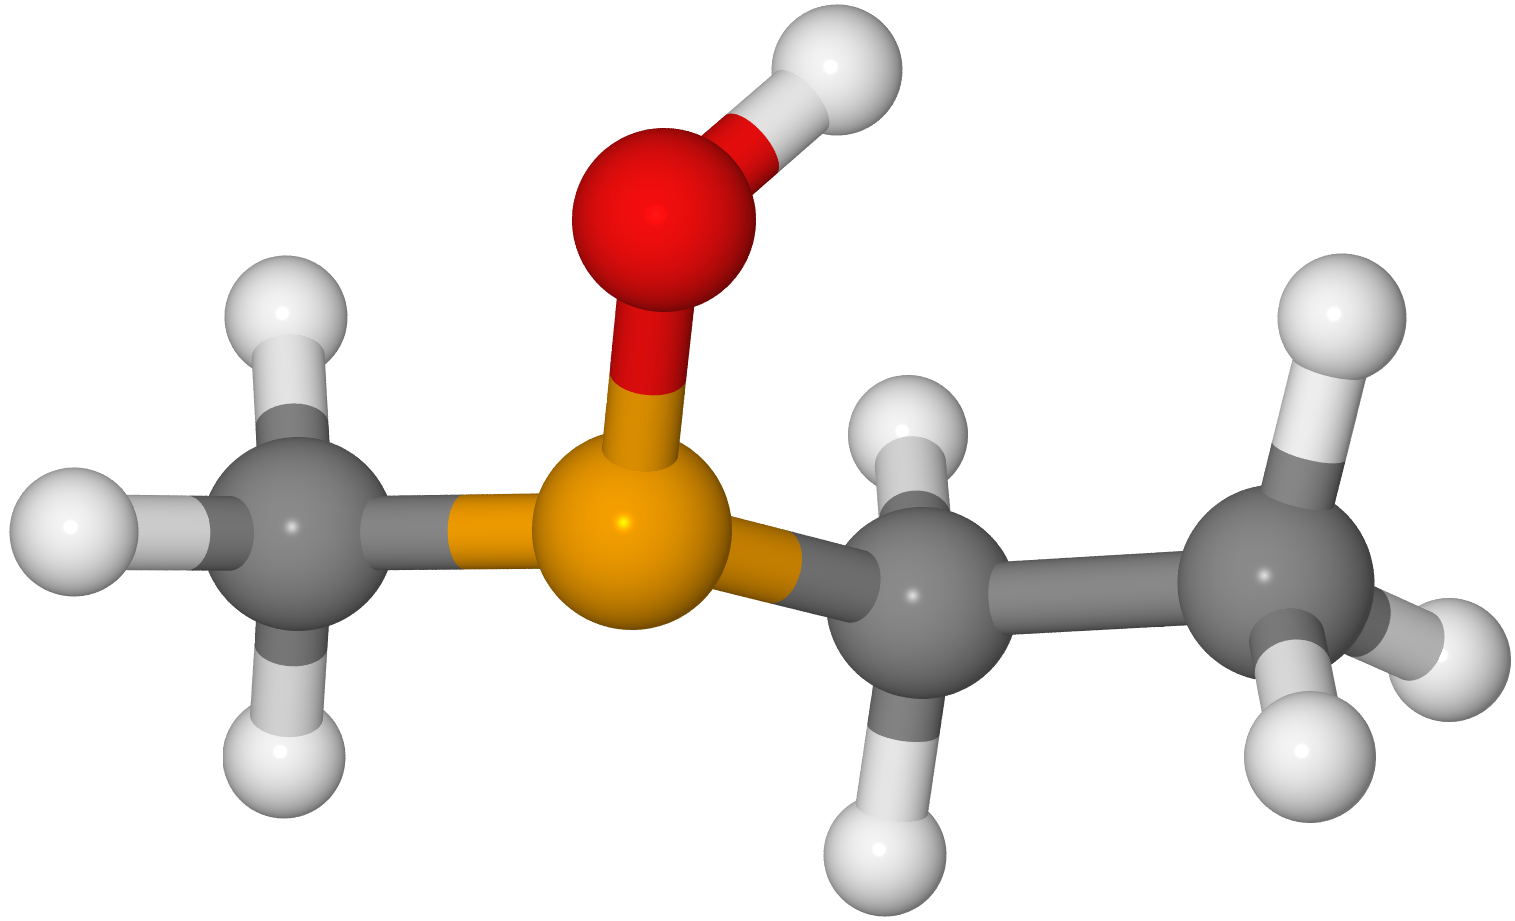
\includegraphics[height=2cm]{03-Butanol/buoh-reactions/sc4h8oh-1}}
    {\Large \textbf{+}}\enspace
    \raisebox{-0.5\height}{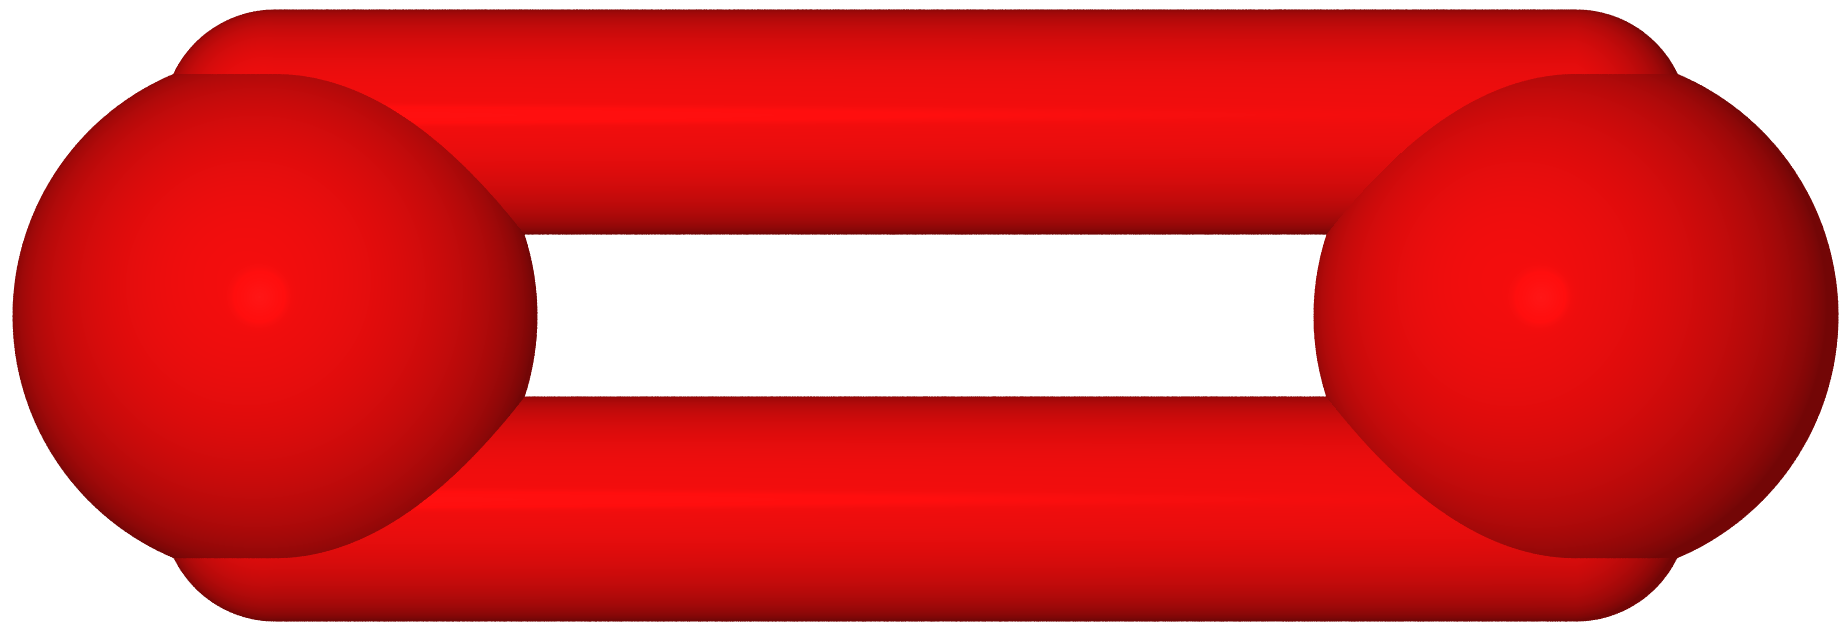
\includegraphics[height=0.5cm]{03-Butanol/buoh-reactions/oxygen}}
    \enspace{\Large \textbf{$\leftrightarrow$}}
    \raisebox{-0.5\height}{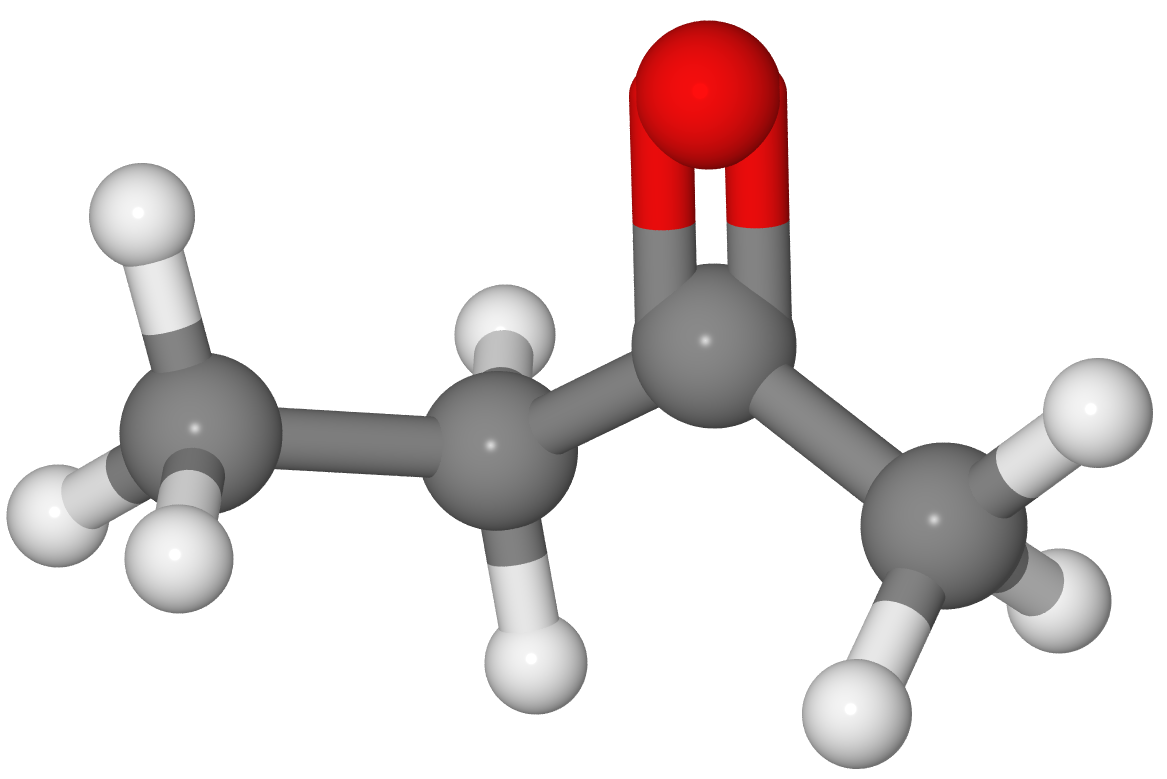
\includegraphics[height=2cm]{03-Butanol/buoh-reactions/2-butanal}}
    {\Large \textbf{+}}\enspace
    \raisebox{-0.5\height}{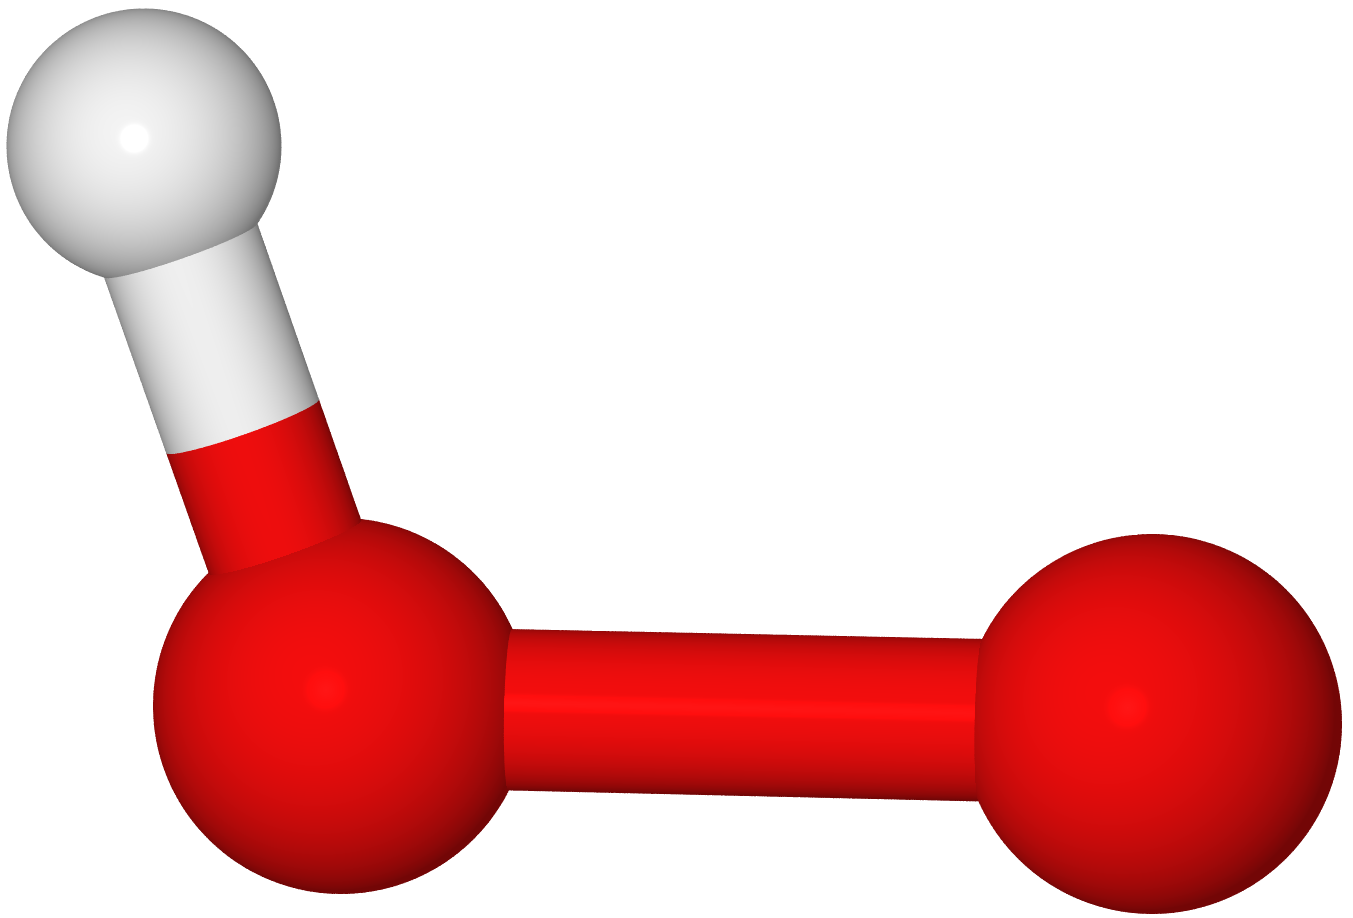
\includegraphics[height=1cm]{03-Butanol/buoh-reactions/hydroperoxy}}

    \blankline

    R4: \quad \raisebox{-0.5\height}{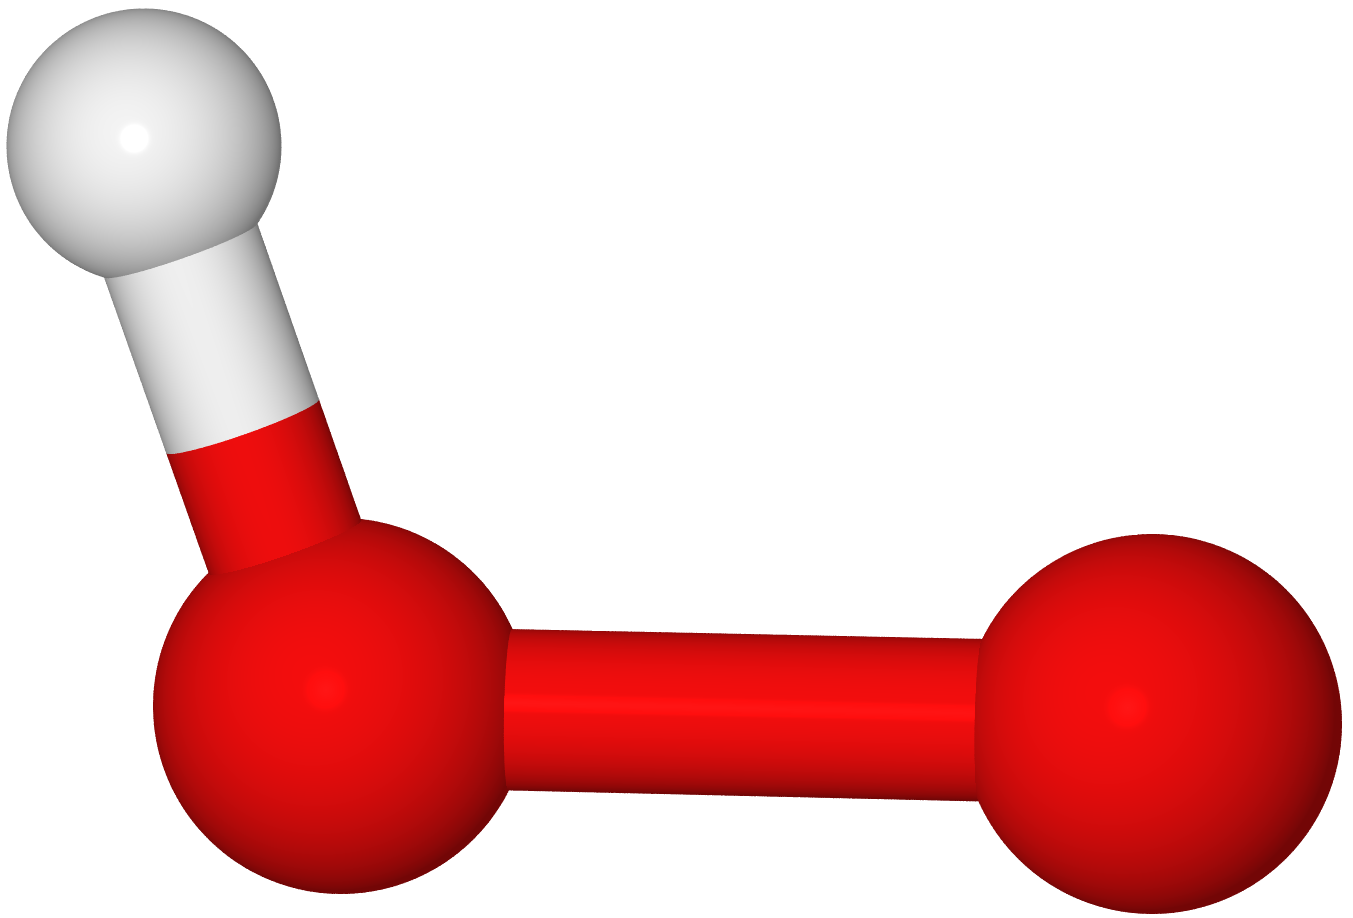
\includegraphics[height=1cm]{03-Butanol/buoh-reactions/hydroperoxy}}
    {\Large \textbf{+}}\enspace
    \raisebox{-0.5\height}{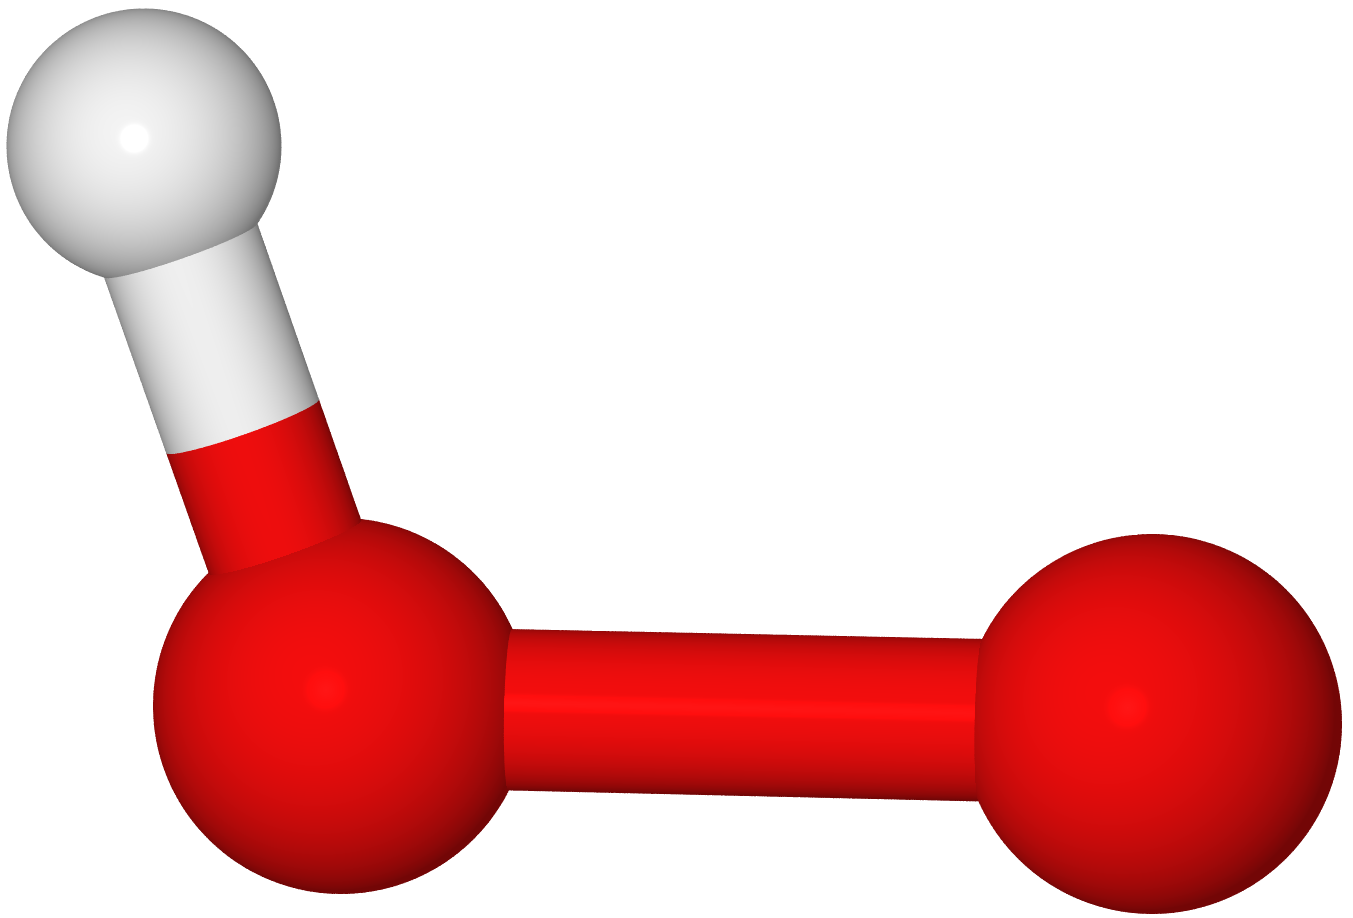
\includegraphics[height=1cm]{03-Butanol/buoh-reactions/hydroperoxy}}
    {\Large \textbf{$\leftrightarrow$}}\enspace
    \raisebox{-0.5\height}{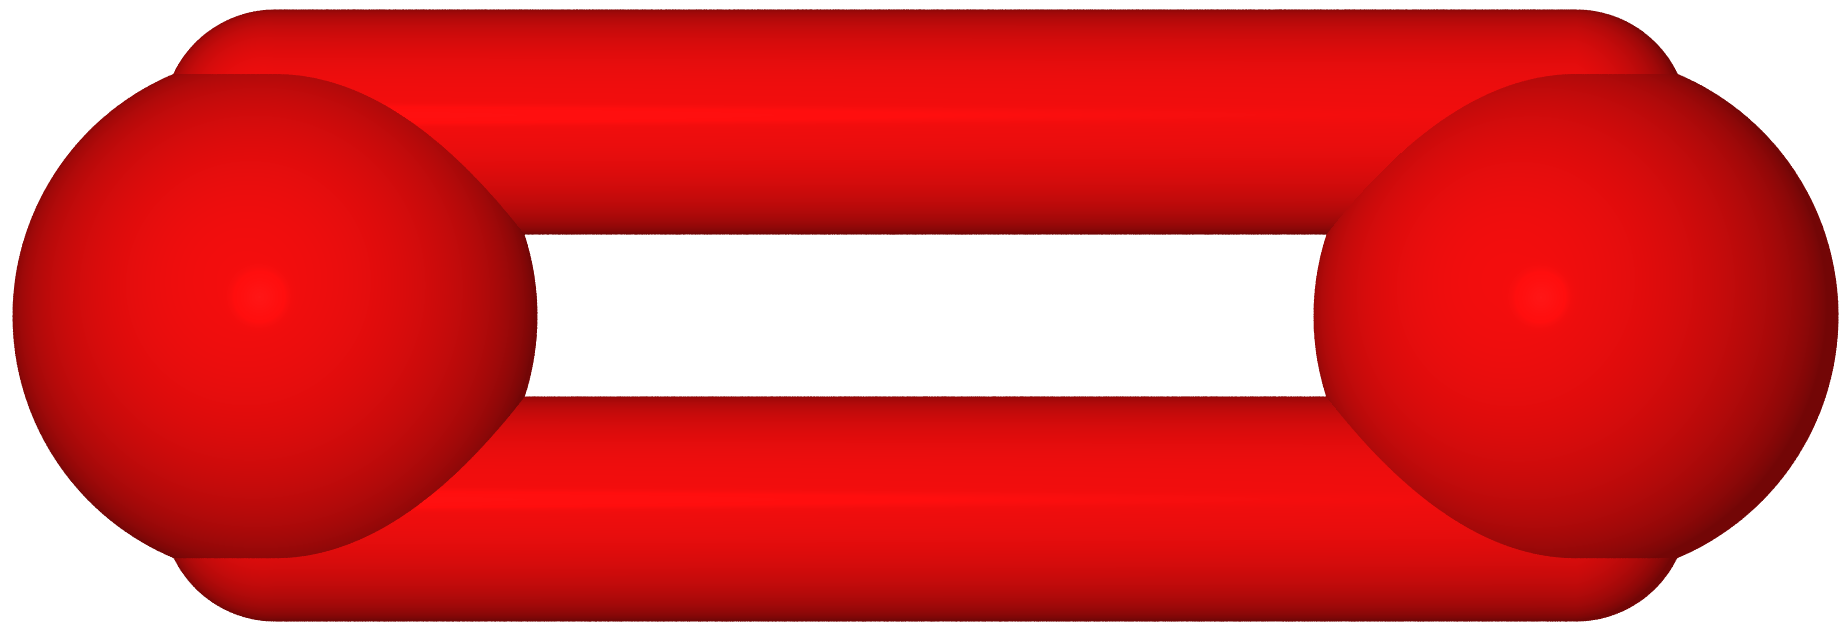
\includegraphics[height=0.5cm]{03-Butanol/buoh-reactions/oxygen}}
    \enspace{\Large \textbf{+}}\enspace
    \raisebox{-0.5\height}{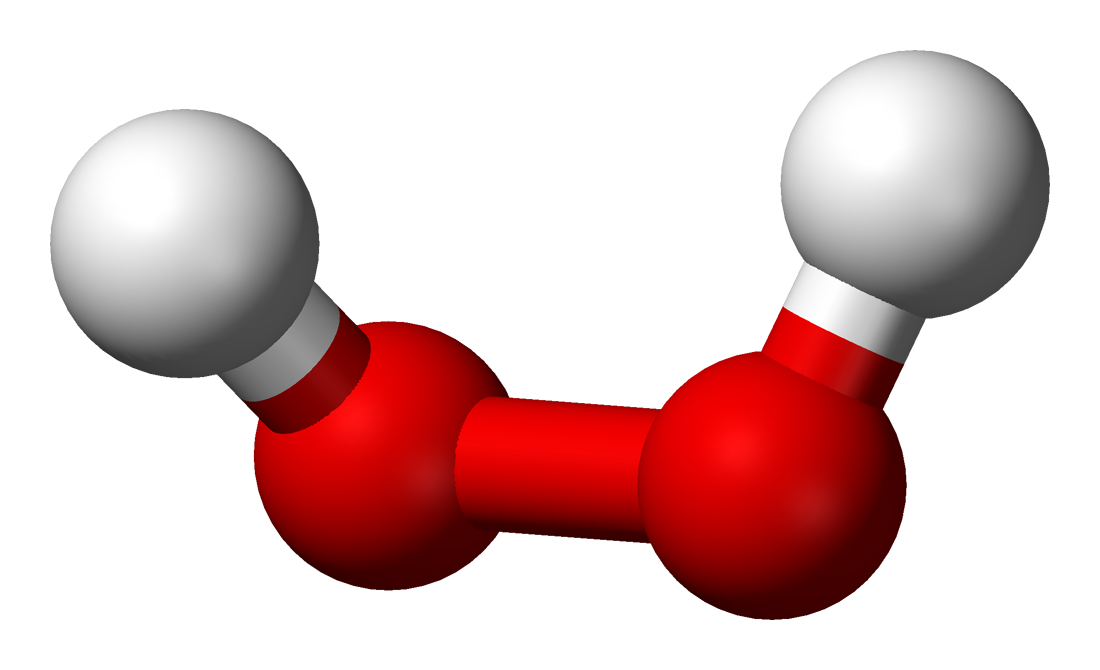
\includegraphics[height=1cm]{03-Butanol/buoh-reactions/hydrogen-peroxide}}

    \caption{Reactions causing the most heat release in the ignition of the
        butanol isomers. The reaction number refers to \cref{fig:buoh-heat}.}
    \label{fig:buoh-reacs}
\end{figure}

Other researchers have also undertaken studies of the low to intermediate
temperature combustion of \tBuOH{}. \textcite{Lefkowitz2012}
performed a study in the Variable Pressure Flow Reactor (VPFR) at Princeton
University on the oxidation of \tBuOH{} over the temperature range
from \SIrange{680}{950}{\kelvin}, at \SI{12.5}{atm} and stoichiometric mixture conditions. It is
interesting to note that they found no evidence of traditional hydrocarbon
low temperature chemistry. They did, however, find significant quantities of
acetone, peaking at approximately \SI{800}{\kelvin}. \textcite{Lefkowitz2012} concluded
that the primary pathways of acetone formation are tautomerization of
propen-2-ol and $\beta$-scission of the alkoxy radical, based on an analysis
of the mechanism from \textcite{Grana2010}. Both of these pathways are
dependent on unimolecular decomposition of the hydroxybutyl radicals. However,
this mechanism has only been validated for flame studies; indeed, an updated
version of this model (by \textcite{Frassoldati2012}) is unable to predict the
low-temperature ignition delays measured in this study and hence is not
considered for analysis.

In contrast to the study of \textcite{Lefkowitz2012}, path analysis of the
mechanism by \textcite{Sarathy2012} shows that unimolecular decomposition
of the hydroxybutyl radicals is not the most important pathway; as mentioned
earlier, the most important pathway is the formation of
$\beta$-hydroxybutylperoxy. Further analysis shows that the primary pathway of
reaction of the \tBuOH{} $\beta$-hydroxybutylperoxy species is
through the Waddington mechanism. The Waddington mechanism has been shown
experimentally to be an important pathway for $\beta$-hydroxypentylperoxy
radicals in the low temperature combustion of \textit{i}-pentanol
\cite{Welz2012}, as well as the $\beta$-hydroxybutylperoxy radicals of
\textit{i}- and \tBuOH{} \cite{Welz2013b}. \textit{t}-Butanol only
produces $\beta$-hydroxybutyl radicals, and one of the products of the
Waddington pathway in \tBuOH{} is acetone (the others are
formaldehyde and hydroxyl radical); over \SI{88}{\percent} of the acetone produced up to the
\SI{20}{\percent} fuel consumption point is produced by the Waddington reaction. The study
in the VPFR thus provides further evidence of the importance of low-temperature
hydroxybutylperoxy chemistry in \tBuOH{}, although it is not
traditional hydrocarbon low-temperature chemistry.

Up to this point, the discussion has focused mainly on the importance of
hydroxybutylperoxy chemistry in \tBuOH{}. Nevertheless, the chemistry
of the hydroxybutylperoxy species is important in the combustion of the other
isomers of butanol as well. Using the high pressure ST at RWTH Aachen
University, \textcite{Vranckx2011} showed the importance of peroxy chemistry
pathways in the autoignition of \nBuOH{}. By adding a lumped peroxy
model to an existing kinetic model for \nBuOH{} combustion, they were
able to substantially improve agreement of the model with their experiments at
high pressure and low temperature \cite{Vranckx2011}.

\subsection{Comparison of \textit{i}-Butanol Mechanisms}
\label{sec:ibuoh-discussion}

As discussed in \cref{sec:ibuoh-sims}, the Sarathy et al.\ mechanism
\cite{Sarathy2012} tends to under-predict the experimental ignition
delays of \iBuOH{}, whereas the MIT mechanism \cite{Weber2013a} tends to
over-predict the experimental data. Some of the differences between the
mechanisms are demonstrated by the path flux diagram shown in
\cref{fig:ibuoh-mitpath}. The diagram is produced by the same procedure
as \crefrange{fig:buoh-npath}{fig:buoh-ipath}, except the initial
conditions of the simulation considered in \cref{fig:ibuoh-mitpath} are
\SI{810}{\kelvin} and \SI{30}{\bar} for a stoichiometric mixture of
\iBuOH{} with air. The percentages in plain text are the results from a
simulation with the MIT mechanism \cite{Weber2013a}; the percentages in
italics are from a simulation with the Sarathy et al.\ mechanism
\cite{Sarathy2012}.

\begin{figure}
    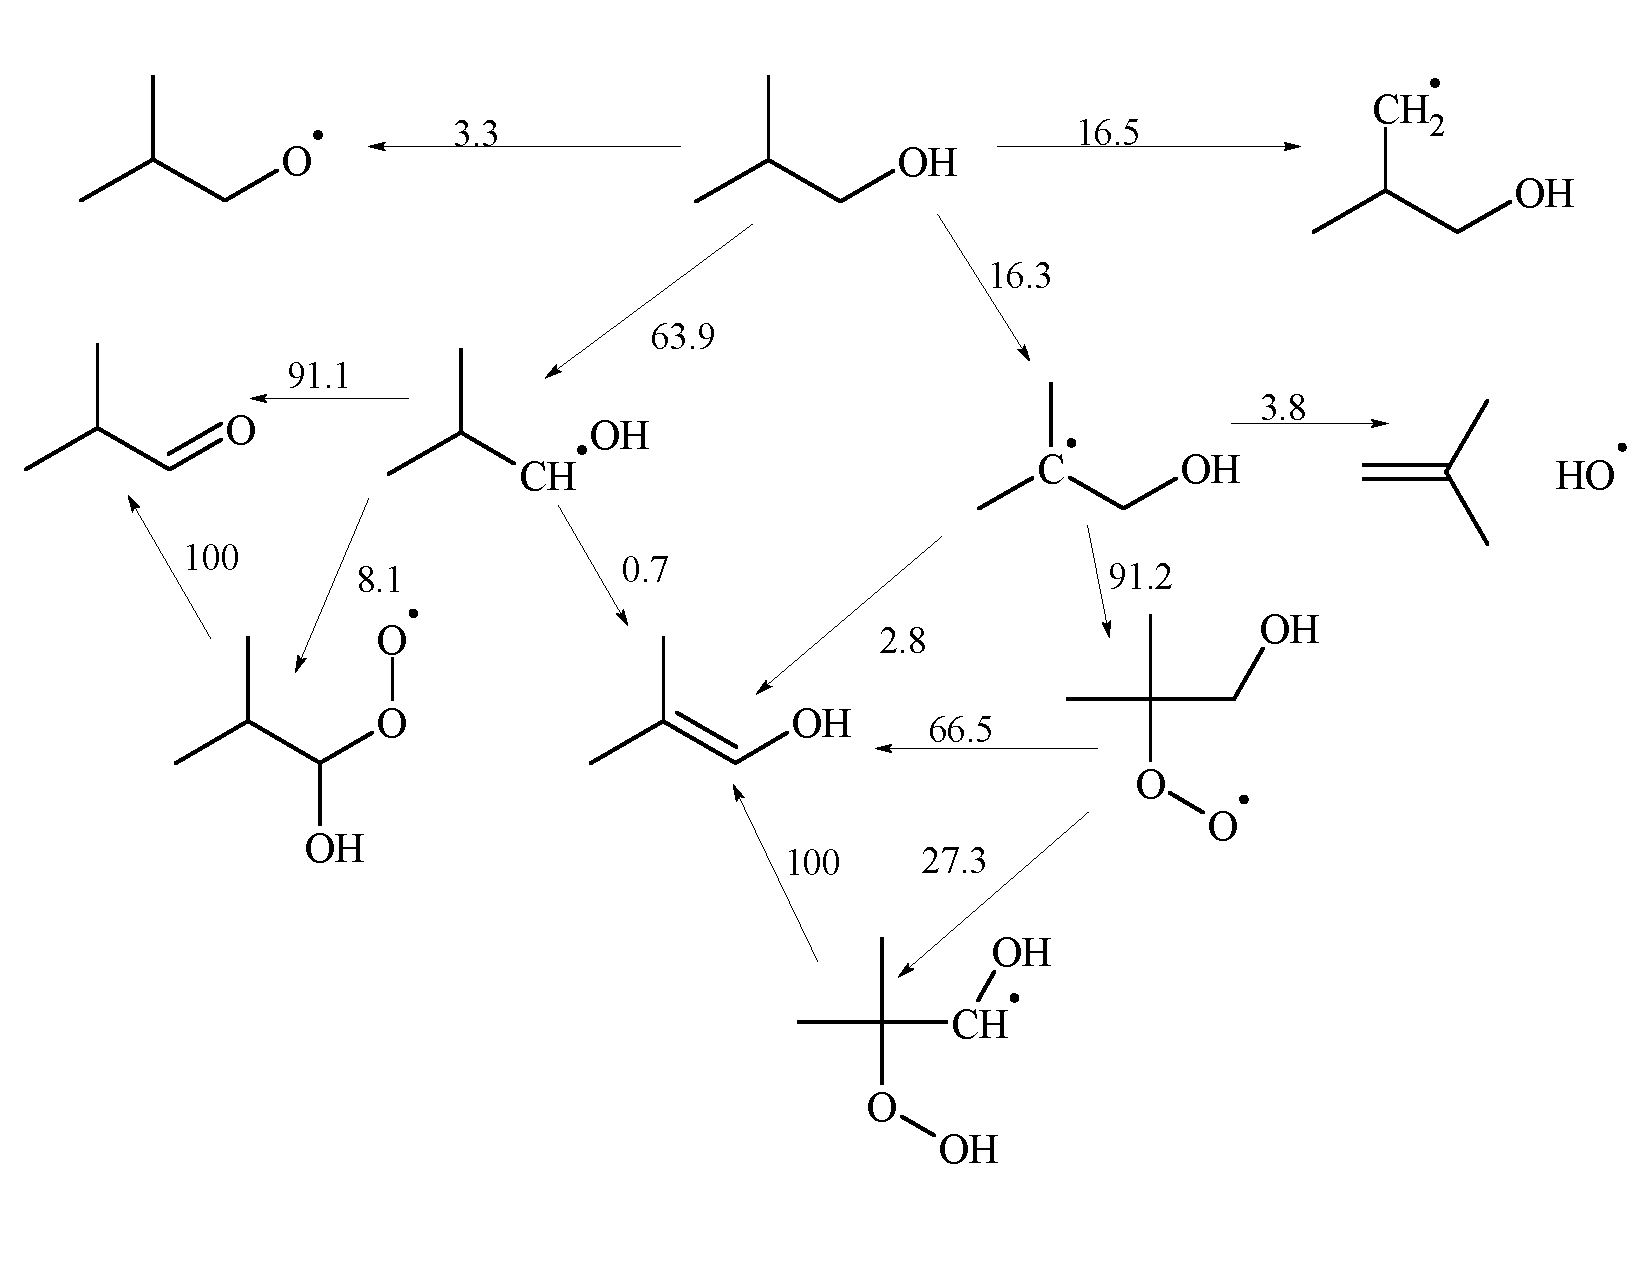
\includegraphics[width=12cm]{03-Butanol/ibuoh-mitpath}
    \caption{Path flux diagram for \iBuOH{}/O$_2$/N$_2$, $\phi=1.0$,
    \SI{810}{\kelvin}, \SI{30}{\bar}. Plain text indicates the MIT
    mechanism \cite{Weber2013a}; italic text indicates the Sarathy et al.\ mechanism
    \cite{Sarathy2012}.}
    \label{fig:ibuoh-mitpath}
\end{figure}

Only the pathways for the $\alpha$- and $\beta$-hydroxybutyl radicals
are shown in \cref{fig:ibuoh-mitpath}; analysis of the $\gamma$-hydroxybutyl
and isobutoxy radicals shows similar important pathways for both mechanisms.
\Cref{fig:ibuoh-mitpath} shows that there is a good agreement between
the mechanisms in the first step of fuel decomposition, although the MIT
mechanism tends to form slightly more $\beta$-hydroxybutyl and slightly
less $\alpha$-hydroxybutyl than the Sarathy et al.\ mechanism. The
subsequent reactions of the primary fuel radicals are also similar
between the mechanisms, although the formation of $\alpha$- and
$\beta$-hydroxybutylperoxy occurs more frequently in the Sarathy et al.\
mechanism than in the MIT mechanism.

However, larger differences between the models are evident in the third level
of reactcions. In the pathway of the $\beta$-hydroxybutyl radical, the breakdown
of the $\beta$-hydroxybutylperoxy radical occurs partially via the Waddington
mechanism to form acetone, formaldehyde and hydroxyl radical (OH) in the
Sarathy et al.\ mechanism, whereas this pathway is not active in the
MIT mechanism. This pathway is included in the MIT model but is not
active under the conditions of this simulation.

Moreover, the fate of the $\alpha$-hydroxybutylperoxy species is
among the most important pathways in controlling the reactivity of the
model and shows significant differences between the models. In the MIT
mechanism, nearly all of the $\alpha$-hydroxybutylperoxy goes to form
isobutyraldehyde, which is itself the primary product of reactions of
$\alpha$-hydroxybutyl. This means that over \SI{99}{\percent} of the
$\alpha$-hydroxybutyl radical is directed into the formation of
isobutyraldehyde and hydroperoxyl (HO$_2$) in the MIT mechanism.
However, in the Sarathy et al.\ mechanism, only about a quarter of the
$\alpha$-hydroxybutylperoxy goes to form isobutyraldehyde, and the rest
is directed into traditional hydrocarbon low-temperature chain branching
pathways leading to the formation of the hydroxyl radical.

The pathways involving $\alpha$-hydroxybutyl and its products is of
critical importance because the radical species produced from these
pathways control the reactivity of the model. In the mechanism of
\textcite{Sarathy2012}, the radical that primarily controls \iBuOH{}
decomposition is hydroxyl, whereas in the MIT model \cite{Weber2013a},
the reactivity is controlled by the hydroperoxyl radical.

In their work, \textcite{Sarathy2012} used the reaction rates computed by
\textcite{DaSilva2009} for the hydroxyethyl system (i.e.\ ethanol as the parent
fuel) to determine the rate of direct reaction of $\alpha$-hydroxybutyl and
oxygen to form aldehyde and HO$_2$, and then set the rate of oxygen addition to
the $\alpha$-hydroxybutyl radical (to form $\alpha$-hydroxybutylperoxy) so that
the total rate was less than the collisional limit. The rates of oxygen
addition for the other radicals were prescribed depending on the type of carbon
(primary, secondary, or tertiary) based on studies of butane and
\textit{i}-octane \cite{Sarathy2012}. Based on the well-known importance of
hydroxyl in driving the reactivity of combustion systems, and the sources of
the estimates for the reaction rates of oxygen addition to hydroxybutyl (i.e.
the entry to the pathway that controls the rate of hydroxyl formation), it can
be hypothesized that the rates of hydroxybutylperoxy formation are
overestimated in the mechanism of \textcite{Sarathy2012}, as the simulated
results under-predict the experimental data of \iBuOH{}.

This hypothesis is supported by the results shown in \cref{fig:buoh-sens},
which shows the linear brute force sensitivity of the ignition delay ($\tau$)
of \iBuOH{} with respect to changes in the $\mathrm{A}$-factor of the rate coefficient, using
the mechanism from \textcite{Sarathy2012}. The percent sensitivity is defined
as the difference between the ignition delay when the $\mathrm{A}$-factor of each reaction
is halved and the nominal ignition delay, normalized by the nominal ignition
delay, as shown below:

\begin{equation}
    \label{eq:buoh-sens}
    S_i=\frac{\tau(0.5\mathrm{A}_i )-\tau(\mathrm{A}_i )}{\tau(\mathrm{A}_i)} \times \SI{100}{\percent}
\end{equation}

Therefore, negative sensitivity means that halving the $\mathrm{A}$-factor of a reaction
decreases the ignition delay, and positive sensitivity indicates the ignition
delay increases. These results are for CONV simulations with initial conditions
of \SI{750}{\kelvin} and \SI{30}{\bar} as well as \SI{1200}{\kelvin} and \SI{30}{\bar}.

\begin{figure}
    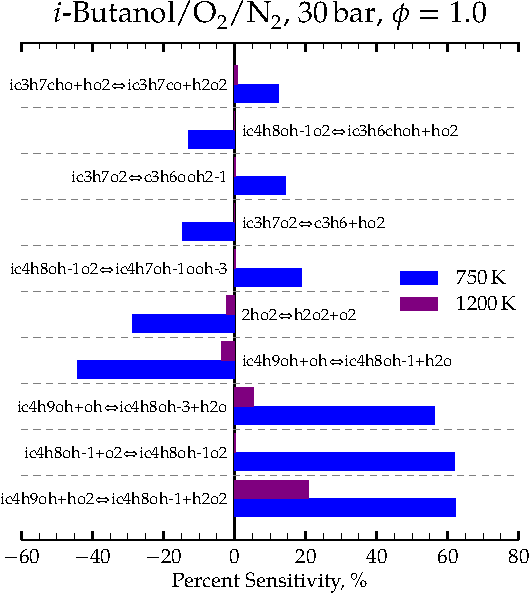
\includegraphics[width=10cm]{03-Butanol/buoh-sens}
    \caption{Linear brute force sensitivity analysis of the ignition delay with
        respect to the A-factors of the listed reactions in the mechanism from
        \textcite{Sarathy2012}. Positive quantities indicate the ignition delay
        is increased when the $\mathrm{A}$-factor is halved.}
    \label{fig:buoh-sens}
\end{figure}

The most sensitive reaction at the lower temperature is the initiation reaction
of the fuel with hydroperoxyl radical to form the primary fuel radical and the
second most sensitive reaction is the addition of oxygen to the primary
radical. Both of these reactions have positive sensitivities, indicating that
reducing the rate of these reactions increases the ignition delay
and improves the agreement of the simulations relative to the experiments
in this case. It is apparent, then, that reducing the amount of fuel
propagating into the low temperature chain branching pathway of oxygen
addition to the primary $\alpha$-radical improves the simulated results.
Interestingly, the \iBuOH{} system is not sensitive to the rates of
oxygen addition to the hydroxybutyl radicals other than the
$\alpha$-radical. At the higher temperature of \SI{1200}{\kelvin}, there
is little sensitivity on the ignition delay by changing the rate of the
oxygen-addition reaction, demonstrating its lack of influence at higher
temperatures.

As a final comparison, we have modified this pathway in the mechanism from
\textcite{Sarathy2012} so that the rate of oxygen addition to the primary
fuel radical is arbitrarily set to zero; that is, the rate of the reaction
ic4h8oh-1+o2=ic4h8oh-1o2 is set to zero by zeroing the $\mathrm{A}$-factor, while the
rates of the other oxygen addition reactions were unchanged. This unphysical
situation substantially changes the results of simulations for
\iBuOH{}---removing this pathway in the mechanism from
\textcite{Sarathy2012} brings the simulations into close agreement with the
ignition delay results from the MIT mechanism. In the MIT mechanism, the
reactions of $\alpha$-hydroxybutylperoxy exclusively produce
\textit{i}-butyraldehyde, whereas in the Sarathy et al.\ mechanism, some
of the $\alpha$-hydroxybutylperoxy radicals enter chain-branching
pathways. Since the other oxygen addition reactions were unchanged, it
is apparent that the addition of oxygen to $\alpha$-hydroxybutyl is one
of the controlling reactions for the high-pressure, low-temperature
ignition of \iBuOH{} using the mechanism of \textcite{Sarathy2012}. It
is therefore concluded that a detailed examination of the rates of
direct formation of aldehyde+HO$_2$ and oxygen addition to the
$\alpha$-hydroxybutyl radical are required to better predict the
low-temperature ignition behavior of \iBuOH{}. Furthermore, based on the
other results of this study, a detailed analysis of the oxygen addition
reactions to all the isomers of butanol is probably warranted.

\section{Conclusions}
\label{sec:buoh-conclusions}

In this work, ignition delays for all four isomers of butanol in stoichiometric
mixture with air are presented over the low to intermediate temperature
range, and at two compressed pressures of \SIlist{15;30}{\bar}. The order of
reactivity of the isomers, in terms of the inverse of the ignition delay,
is \nBuOH{}$>$\sBuOH{}$\approx$\iBuOH{}$>$\tBuOH{}
at the lower pressure, but changes to \nBuOH{}$>$\tBuOH{}$>$\sBuOH{}$>$\iBuOH{}
at the higher pressure. This unexpected result is partially explained by
the fact that there is substantial pre-ignition heat release present
for \tBuOH{}. To help understand the nature of the pre-ignition heat
release of \tBuOH{}, studies at off-stoichiometric conditions,
$\phi=\num{0.5}$ and $\phi=\num{2.0}$ in air, are also conducted. Finally,
ignition delays are collected for a $\phi=\num{0.5}$ mixture of \iBuOH{}
in air as well as $\phi=\numlist{0.5;1.0;2.0}$ mixtures where the initial
fuel mole fraction is held constant.

Comparisons of the experimentally measured ignition delays with two kinetic
mechanisms show good agreement for certain isomers, but relatively poorer
agreement for others. The kinetic mechanism of \textcite{Sarathy2012} is used
to further elucidate the chemical processes controlling the autoignition of
these butanol isomers. Pathway analysis of the fuel decomposition shows that
\textit{n}-, \textit{s}-, and \iBuOH{} primarily form
$\alpha$-hydroxybutyl radicals, because the proximity of the $\alpha$ carbon to
the hydroxyl group reduces the C-H bond energy. The $\alpha$-hydroxybutyl radicals
tend to form an aldehyde plus HO$_2$  directly, without forming a
hydroxybutylperoxy complex. However, due to its unique structure,
\tBuOH{} can only form $\beta$-radicals; these radicals do not have
the tendency to react with oxygen to directly form HO$_2$  and an aldehyde.
Rather, \tBuOH{} preferentially adds oxygen to the fuel radical site.
It is hypothesized that this reaction, O$_2$  addition to form
hydroxybutylperoxy, causes the pre-ignition heat release in \tBuOH{}
and leads to a chain propagation pathway through the Waddington mechanism. The
fact that this oxygen-addition reaction is preferred is unique to
\tBuOH{}, although a detailed understanding of the peroxy chemistry
of alcohols is still of vital importance to the other butanol isomers. This is
further demonstrated in this work for the case of \iBuOH{}, where the
ignition delay is quite sensitive to both the rate of primary fuel
radical formation and to the rate of oxygen addition to the primary fuel
radical. It is also noted that \nBuOH{} autoignition was
quite sensitive to peroxy chemistry in the study of \textcite{Vranckx2011}.

All together, these analyses show the importance of the peroxy chemistry
pathways in the autoignition of the butanols. Further experimental studies,
such as species profiles from the low temperature ignition of the butanol
isomers, could help reduce uncertainty in the pathways of fuel breakdown.
Finally, further understanding of the rates of the peroxy pathways is
important and therefore further theoretical and quantum chemical studies are
warranted.

\end{document}
